\chapter{Intervalos de confianza}

\section{Intervalos de confianza}

\begin{definicion}[65 --- $\alpha$-cuantiles]
Sea $X$ una v.a.\ continua con función de distribución $F$. Si $p \in (0,1)$, el $p$-cuantil, denotado por $Q(p)$ o $Q_p$, es
\[
  Q_p = \inf\{x : F_X(x) = p\} = F_X^{-1}(p).
\]\textcolor{blue}{
Si $X$ no es necesariamente una v.a.\ continua, $F_X$ no define una función biyectiva en $[0,1]$ y la ecuación anterior puede no tener solución; en ese caso definimos
\[
  Q_p = \inf\{x : F(x) \ge p\}.
\]
Similarmente se definen los cuantiles de cola:
\[
  z_p = \inf\{x : \overline{F}(x) \equiv \Prob(X \ge x) = p\} \iff z_p \equiv \overline{Q}_p \coloneqq \overline{F}^{-1}(p) = F^{-1}(1-p) \equiv Q_{1-p}.
\]}
\end{definicion}
\begin{definicion}[66 --- Intervalo de confianza para variables aleatorias]
Dado un nivel de confianza $\alpha$, normalmente $\alpha = 0{,}95$, un intervalo de confianza para la v.a.\ $X$ es el intervalo $I = (a_-, a_+)$ tal que
\[
  \Prob(X \in I) = \alpha \iff F_X(a_+) - F_X(a_-) = \alpha.
\]
Nótese que tenemos dos incógnitas $a_-, a_+$ y una única ecuación para determinarlos (problema indeterminado). Hay diferentes elecciones posibles para fijar una de las dos como función de la otra.
\end{definicion}

\begin{proposicion}[85 --- Intervalos simétricos o estándar] \, 
\begin{enumerate}
  \item Si se requiere que
  \[
    F_X(a_-) \equiv \Prob(X \le a_-) = \Prob(X \ge a_+) \equiv 1 - F_X(a_+) = \frac{1-\alpha}{2},
  \]
  el intervalo de confianza satisface $2F_X(a_+) - 1 = \alpha$ y viene definido por
  \[
    F_X(a_\pm) = \frac{1 \pm \alpha}{2}; \qquad a_\pm = F_X^{-1}\left(\frac{1 \pm \alpha}{2}\right) \equiv Q_{(1\pm\alpha)/2}.
  \]
  \item Si $f$ es simétrica respecto al origen, $f(x) = f(-x) \iff F_X(x) = 1 - F_X(-x)$, entonces
  \[
    a_- = -a_+ = -F_X^{-1}\left(\frac{1+\alpha}{2}\right).
  \]
  \item Si $X \sim \mathcal{N}(0,1)$, el i.c.\ es $(-a_+, a_+)$ donde
  \[
    -a_- = a_+ = \Phi^{-1}\left(\frac{1+\alpha}{2}\right).
  \]
  En particular, si $X \sim \mathcal{N}(0,1)$ y $\alpha = 0{,}95$, entonces $Q_{(1+\alpha)/2} = 1{,}96$ y el intervalo $I = (-1{,}96,\, 1{,}96)$ contiene el $95\%$ de probabilidad: $\Prob(X \in I) = 0{,}95$.
  \item Si $X \sim \mathcal{N}(\mu, \sigma^2)$, el intervalo de confianza con nivel $\alpha$ es
  \[
    a_\pm = \mu \pm \sigma\,\Phi^{-1}\left(\frac{1+\alpha}{2}\right).
  \]
  \item Si $X \sim \mathcal{N}(\mu, \sigma^2)$, el intervalo $\mu \pm \sigma\lambda$ corresponde a un nivel de confianza
  \[
    \alpha = 2\Phi(\lambda) - 1 \quad \left(\iff \lambda = \Phi^{-1}\left(\frac{1+\alpha}{2}\right)\right).
  \]
  En particular, $\alpha = 0{,}68,\ 0{,}95\ \text{y}\ 0{,}99$ para $\lambda = 1, 2, 3$.
\end{enumerate}
\end{proposicion}

\begin{proof}
Sea $N \coloneqq (X - \mu)/\sigma \sim \mathcal{N}(0,1)$. Llamando $(a_+ - \mu)/\sigma \coloneqq z$ tenemos
\begin{align*}
  \Prob(a_- \le X \le a_+) &= \Prob\left(\frac{a_- - \mu}{\sigma} \le N \le \frac{a_+ - \mu}{\sigma}\right) \\
  &= 2\Prob\left(N \le \frac{a_+ - \mu}{\sigma}\right) - 1 \equiv 2\Phi(z) - 1 = \alpha \\
  &\iff z = \Phi^{-1}\left(\frac{1+\alpha}{2}\right) \iff a_\pm = \mu \pm \sigma\,\Phi^{-1}\left(\frac{1+\alpha}{2}\right). \qedhere
\end{align*}
\end{proof}

\begin{proposicion}[86]
Supongamos que $X$ tiene dos momentos finitos ($\sigma < \infty$). El intervalo $(a_-, a_+)$ donde $a_\pm = \mu \pm \lambda\sigma$ es un intervalo de confianza con nivel $\ge 1 - 1/\lambda^2$ al menos.
\end{proposicion}

\begin{proof}
Por la desigualdad de Chebyshev:
\[
  \Prob\bigl(X \notin (a_-, a_+)\bigr) = \Prob(|X - \mu| \ge \lambda\sigma) \le \frac{\sigma^2}{\lambda^2\sigma^2} = \frac{1}{\lambda^2}\]
  \[
  \implies \Prob\bigl(X \in (a_-, a_+)\bigr) = \Prob(|X - \mu| < \lambda\sigma) \ge 1 - \frac{1}{\lambda^2}. \qedhere
\]
\end{proof}

\begin{proposicion}[87]
Sea $(a_-, a_+)$ el intervalo de confianza para $X$ a nivel $\alpha$. Sea $g : \R \to \R$ estrictamente creciente. Un intervalo de confianza para $Y \coloneqq g(X)$ a nivel $\alpha$ es $(g(a_-), g(a_+))$.
\end{proposicion}\begin{figure}[htbp]
  \centering
  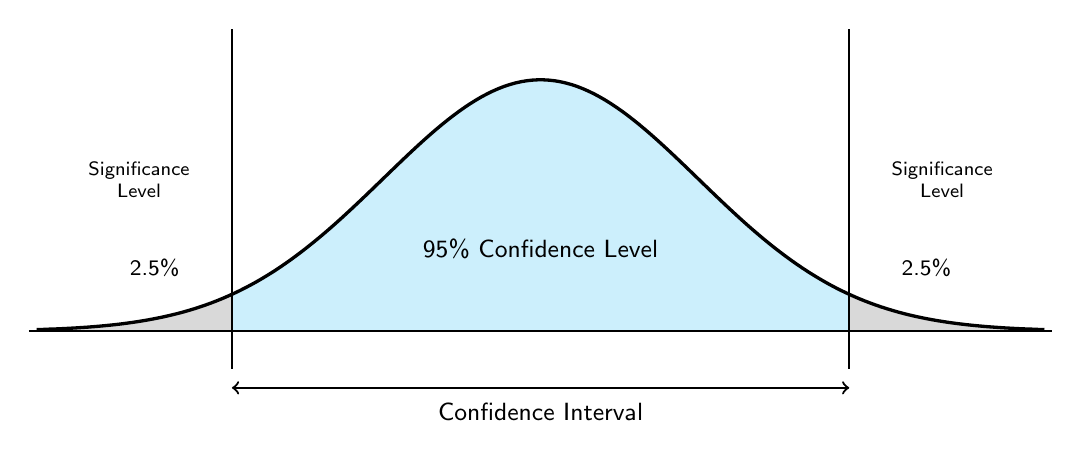
\begin{tikzpicture}[x=2cm, y=8cm]
    % Curva normal estándar escalada visualmente para buena proporción
    \def\gauss#1{exp(-0.5*(#1)^2)/sqrt(2*pi)}

    % Área central (95% Confidence Level)
    \fill[cyan!20, domain=-1.96:1.96, samples=120]
      (-1.96, 0) -- plot (\x, {\gauss{\x}}) -- (1.96, 0) -- cycle;

    % Colas laterales (2.5% cada una)
    \fill[gray!30, domain=-3.2:-1.96, samples=80]
      (-3.2, 0) -- plot (\x, {\gauss{\x}}) -- (-1.96, 0) -- cycle;
    \fill[gray!30, domain=1.96:3.2, samples=80]
      (1.96, 0) -- plot (\x, {\gauss{\x}}) -- (3.2, 0) -- cycle;

    % Eje base y curva
    \draw[thick] (-3.25, 0) -- (3.25, 0);
    \draw[very thick, domain=-3.2:3.2, samples=180] plot (\x, {\gauss{\x}});

    % Líneas verticales en los cuantiles +-1.96
    \draw[thick] (-1.96, -0.06) -- (-1.96, 0.48);
    \draw[thick] (1.96, -0.06) -- (1.96, 0.48);

    % Etiquetas interiores
    \node[font=\sffamily\small] at (0, 0.13) {95\% Confidence Level};
    \node[font=\sffamily\footnotesize] at (-2.45, 0.1) {2.5\%};
    \node[font=\sffamily\footnotesize] at (2.45, 0.1) {2.5\%};
    \node[font=\sffamily\scriptsize, align=center] at (-2.55, 0.24) {Significance\\Level};
    \node[font=\sffamily\scriptsize, align=center] at (2.55, 0.24) {Significance\\Level};

    % Flecha del intervalo de confianza
    \draw[<->, thick] (-1.96, -0.09) -- (1.96, -0.09)
      node[midway, below=2pt, font=\sffamily\small] {Confidence Interval};
  \end{tikzpicture}
  \caption*{Figura 2. Intervalo de confianza para $X$ a nivel $\alpha = 0{,}95$.}
  \label{fig:ic-95}
\end{figure}

\section{Estimación de intervalo de confianza para un estimador $\Theta$}

El intervalo de confianza para un estimador se define de forma exactamente igual considerando la FdD del estimador:

\begin{definicion}[67 --- Intervalo de confianza para estadísticos]
Dado un nivel $\alpha$, un intervalo de confianza para el estadístico $\Theta_n = T(X_1, \dots, X_n)$ es el intervalo real $I_n = (a_-, a_+)$ tal que
\[
  \Prob(\Theta_n \in I_n) = \alpha \iff F_{\Theta_n}(a_+) - F_{\Theta_n}(a_-) = \alpha.
\]
Si se requiere que
\[
  F_{\Theta_n}(a_-) = 1 - F_{\Theta_n}(a_+) = \frac{1-\alpha}{2}
  \implies F_{\Theta_n}(a_\pm) = \frac{1\pm\alpha}{2} \implies a_\pm = F_{\Theta_n}^{-1}\left(\frac{1\pm\alpha}{2}\right) \equiv Q_{(1\pm\alpha)/2}.
\]
\end{definicion}

\begin{definicion}[68 --- Condición $n$]
Decimos que $(X_k)_{k=1,\dots,n}$ satisfacen la \emph{condición $n$} si $(X_k)_{k=1,\dots,n} \stackrel{\text{i.i.d.}}{\sim} \mathcal{N}(\mu, \sigma^2)$ o bien si $n \to \infty$ (bajo hipótesis de regularidad / TCL).
\end{definicion}

\begin{teorema}[28 --- de Fisher-Cochran]
Supongamos que $(X_k)_{k=1,\dots,n} \stackrel{\text{i.i.d.}}{\sim} \mathcal{N}(\mu, \sigma^2)$ o sino que satisfacen la condición $n$. Entonces:
\begin{enumerate}
  \item La varianza muestral $S_n^2$ y $\overline{X}_n$ son v.a.s independientes: $\overline{X}_n \indep S_n^2$.
  \item $H \coloneqq (\overline{X}_n - \mu)\sqrt{n}/\sigma \sim \mathcal{N}(0,1)$; $\overline{X}_n \sim \mathcal{N}(\mu, \sigma^2/n)$.
  \item Un estadístico pivote es
  \[
    Q^2 \equiv \frac{n-1}{\sigma^2}S_n^2 \sim \chi_{n-1}^2.
  \]
  \item Otro estadístico pivote es
  \[
    P_n \coloneqq \sqrt{n-1}\frac{H}{Q} \equiv \sqrt{n}\frac{\overline{X}_n - \mu}{S_n} \sim t_{n-1}.
  \]
\end{enumerate}
Aquí $\chi_{n-1}^2$ y $t_{n-1}$ son las distribuciones chi-cuadrado y $t$ de Student con $n-1$ grados de libertad (independientes de los parámetros). La distribución $t_n$ de Student con $n$ grados de libertad tiene densidad de probabilidad
\[
  t_n \sim f(t) = k\left(1 + \frac{t^2}{n}\right)^{-(n+1)/2}, \qquad k \equiv \frac{\Gamma\left(\frac{n+1}{2}\right)}{\sqrt{\pi\,n}\,\Gamma\left(\frac{n}{2}\right)},
\]
donde $\Gamma$ es la función gamma. Además, $P_n = g(\overline{X}_n, S_n, \mu, \sigma) = g(\overline{X}_n, S_n, \mu)$ no depende de $\sigma$.
\end{teorema}

\begin{proposicion}[88 --- Intervalo de confianza para la media conocida la varianza]
Supongamos que $(X_k)$ satisfacen la condición $n$. Un $\alpha$-intervalo de confianza para la media muestral $\overline{X}_n$ es
\[
  a_\pm = \mu \pm \frac{\sigma}{\sqrt{n}}\,Q_{(1+\alpha)/2}.
\]
\end{proposicion}

\begin{proof}
Bajo la condición $n$, sabemos que $\overline{X}_n$ es normal con varianza $\sigma^2/n$ (o lo es asintóticamente cuando $n \to \infty$).
\end{proof}

\section{Intervalo de confianza para el parámetro $\theta$}

\begin{observacion}[31]
Si la distribución de $(X_k)$, $\Prob_X$, depende de un parámetro $\theta$, la de $\Theta_n$ también lo hace y el intervalo de confianza para el estadístico depende del parámetro. Si este es desconocido, los valores $a_\pm$ y el i.c.\ serán también desconocidos.

A partir del intervalo de confianza para el estadístico podemos usar lo anterior para: (i) suponiendo $X \sim \Prob_X(\theta)$ conocido, pero (ii) $\theta$ es desconocido; (iii) si además hemos observado los datos $X_1(\omega) \equiv x_1, \dots, X_n(\omega) \equiv x_n$, entonces (iv) estimar y construir un intervalo de confianza para el parámetro $\theta$. Hay por tanto distintos intervalos de confianza: el de la v.a.\ madre $X$, el del estimador y el i.c.\ aleatorio y muestral del parámetro $\theta$.

La idea puede ejemplificarse con $\overline{X}_n$, donde llamando $z = \Phi^{-1}\left(\frac{1+\alpha}{2}\right)$ y $\Sigma = \frac{\sigma}{\sqrt{n}}$ obtenemos:
\[
  \mu - \Sigma z \le \overline{X}_n \le \mu + \Sigma z \iff \overline{X}_n - \Sigma z \le \mu \le \overline{X}_n + \Sigma z;
\]
\[
  \alpha = \Prob(\mu - \Sigma z \le \overline{X}_n \le \mu + \Sigma z) = \Prob(\overline{X}_n - \Sigma z \le \mu \le \overline{X}_n + \Sigma z),
\]
que nos da simultáneamente un i.c.\ para $\overline{X}_n$ y un i.c.\ aleatorio para $\mu$:
\[
  I_{\overline{X}_n}(\mu, \sigma, z) \coloneqq \left(\mu - \frac{\sigma}{\sqrt{n}}z,\, \mu + \frac{\sigma}{\sqrt{n}}z\right) \quad \text{y} \quad I_{\mu}(\overline{X}_n, \sigma, z) \coloneqq \left(\overline{X}_n - \frac{\sigma}{\sqrt{n}}z,\, \overline{X}_n + \frac{\sigma}{\sqrt{n}}z\right),
\]
y es posible en esta igualdad sustituir $\overline{X}_n$ por su valor observado $\overline{X}_n(\omega) = \overline{x}_n$ y obtener un i.c.\ muestral 
$$(\overline{x}_n - \Sigma z,\, \overline{x}_n + \Sigma z)$$
\end{observacion}

\begin{observacion}[32]
Nótese que el intervalo de confianza del estimador y el del parámetro se obtienen uno de otro cambiando sus roles:
\[
  I_{\mu}(\overline{X}_n, \sigma, z) = \left.I_{\overline{X}_n}(\mu, \sigma, z)\right|_{\mu = \overline{X}_n}.
\]
Se acostumbra a aceptar que esto ocurre siempre, pero en general es falso:
\[
  I_{\theta}(\Theta, z) \neq \left.I_{\Theta}(\theta, z)\right|_{\theta = \Theta}.
\]
Se acostumbra a aceptar también que el i.c.\ del parámetro es de la forma
\[
  I_{\theta}(\Theta, z) = \bigl(\Theta - R(z),\, \Theta + R(z)\bigr)
\]
para cierto $R(z)$, pero en general es falso.
\end{observacion}

\begin{definicion}[69 --- Intervalo de confianza para la media conocida la varianza]
Supongamos que observados los datos $X_1(\omega) \equiv x_1, \dots, X_n(\omega) \equiv x_n$ provenientes de una distribución madre $X \sim \mathcal{N}(\mu, \sigma^2)$: $(X_k)_{k=1,\dots,n} \stackrel{\text{i.i.d.}}{\sim} \mathcal{N}(\mu, \sigma^2)$, donde $\sigma^2$ es conocido pero $\mu$ no. Diremos que $(\overline{x}_n - \Sigma z,\, \overline{x}_n + \Sigma z)$ es un intervalo de confianza para $\mu$.

En un caso general, si $(X_k)^{\text{i.i.d.}}$ satisface las condiciones del TCL, entonces $\frac{\sqrt{n}(\overline{X}_n - \mu)}{\sigma} \xrightarrow{d} \mathcal{N}(0,1)$ cuando $n \to \infty$, donde $\mu \coloneqq \E X_k$, $\sigma^2 = \Var X_k$ se suponen finitas.
\end{definicion}

\begin{definicion}[70]
Un \emph{intervalo de confianza aleatorio} para un parámetro $\theta$ a un nivel $\alpha$ es un conjunto de posibles valores del parámetro dentro del cual se encuentra el verdadero valor del mismo con una probabilidad de $\alpha$. Este conjunto es de la forma
\[
  I \coloneqq \bigl[\Theta_1(X_1, \dots, X_n),\, \Theta_2(X_1, \dots, X_n)\bigr], \qquad \Prob(\theta \in I) = \alpha,
\]
donde $\Theta_1, \Theta_2$ son dos estadísticos. Si realizamos una observación de la muestra $X_1(\omega) \equiv x_1, \dots, X_n(\omega) \equiv x_n$, el intervalo pasa de ser aleatorio a ser un intervalo en la recta real $\bigl[\Theta_1(x_1, \dots, x_n),\, \Theta_2(x_1, \dots, x_n)\bigr]$.
\end{definicion}

\begin{ejemplo}[26]
Se cree que $X \sim \mathcal{N}(\mu, \sigma^2)$ y se sabe que $\sigma = 2$, pero se desconoce $\mu$. En una muestra con $n = 10$ se encuentran los valores
\[
  x_1 = 29{,}0651,\ x_2 = 27{,}3980,\ x_3 = 23{,}4346,\ x_4 = 26{,}3665,\ x_5 = 23{,}4994,
\]
\[
  x_6 = 28{,}6592,\ x_7 = 25{,}5546,\ x_8 = 29{,}4477,\ x_9 = 28{,}0979,\ x_{10} = 25{,}2850.
\]
Aquí $\overline{X}(\omega) = 26{,}68$, $\sigma = 2$, $n = 10$; $z = 1{,}96$ si $\alpha = 0{,}95$ (nivel de significación $0{,}05$). Por tanto:
\[
  I = \left(26{,}68 - 2 \times \frac{1{,}96}{\sqrt{10}},\, 26{,}68 + 2 \times \frac{1{,}96}{\sqrt{10}}\right) = (25{,}44,\, 27{,}92),
\]
es decir, $\mu$ está en ese intervalo con probabilidad del $95\%$. Si $\alpha = 0{,}99 \implies z = 2{,}58$, y $\mu$ está en el intervalo
\[
  I = \left(26{,}68 - 2 \times \frac{2{,}58}{\sqrt{10}},\, 26{,}68 + 2 \times \frac{2{,}58}{\sqrt{10}}\right) = (25{,}10,\, 28{,}26)
\]
con probabilidad del $99\%$.
\end{ejemplo}

\begin{observacion}[33] \,
\begin{enumerate}
  \item Si conocemos $\theta$ y $\Prob_X$, el intervalo de confianza del estimador nos da un intervalo en el cual se encontrarán las observaciones $\Theta(\omega_1), \dots, \Theta(\omega_n)$ con probabilidad $\alpha$.
  \item Si conocemos $\Prob_X$ y la muestra $x_1, \dots, x_n$, y desconocemos $\theta$, el intervalo de confianza para el parámetro $\theta$ nos da un intervalo en el cual se encontrará $\theta$ con probabilidad $\alpha$.
  \item Estos dos intervalos responden a planteamientos distintos y pueden ser muy distintos.
\end{enumerate}
El razonamiento anterior puede usarse para desarrollar un método sistemático para obtener un intervalo de confianza para $\theta$.
\end{observacion}

\begin{definicion}[71 --- Cantidad pivote]
Dada una muestra aleatoria $X_1, \dots, X_n$ dependiente de un parámetro desconocido $\theta$, una \emph{cantidad pivote} (\emph{estadístico pivotal}) es toda $P_n = g(X_1, \dots, X_n, \theta)$ cuya distribución no depende de $\theta$.

La situación estándar es partir de un estadístico $\Theta_n = T(X_1, \dots, X_n)$ cuya distribución $F_{\Theta_n}(x, \theta)$ sí depende de $\theta$ y construir $P_n$ como función de este. El teorema siguiente ilustra la construcción.
\end{definicion}

\begin{teorema}[29 --- Intervalos de confianza aleatorios para el parámetro]
Sea $\theta$ un parámetro y $\Theta_n = T(X_1, \dots, X_n)$ un estimador consistente con distribución $F_{\Theta_n}(x, \theta)$ dependiente de $\theta$. Supongamos que hemos observado los datos $X_1(\omega) \equiv x_1, \dots, X_n(\omega) \equiv x_n$. Supongamos que existe una función de pivote $g : \R \times \R \to \R$, $(x, \theta) \mapsto g(x; \theta)$, satisfaciendo:
\begin{enumerate}
  \item $g(\, \cdot \, ; \theta)$ es una biyección (estrictamente monótona y creciente);
  \item $g(x ; \, \cdot\, )$ es estrictamente decreciente;
  \item $g(x; x) = 0$, $\forall x$;
  \item $P_n \coloneqq g(\Theta_n, \theta) \coloneqq g(T(X_1, \dots, X_n), \theta) \equiv T'(X_1, \dots, X_n, \theta)$ tiene distribución $G(x) \equiv F_{P_n}(x)$ que es independiente de $\theta$ (y de $n$).
\end{enumerate}
Entonces, dado un $\alpha$-valor:
\begin{enumerate}
  \item $C = (c_-, c_+)$ donde $c_\pm = G^{-1}((1\pm\alpha)/2)$ es un intervalo de confianza para $P_n$, independiente de $\theta$:
  \[
    \Prob\bigl(P_n \in (c_-, c_+)\bigr) = \alpha.
  \]
  \item Un intervalo de confianza para el estimador es el intervalo $A = (a_-, a_+)$ donde $g_1^{-1}$ representa la inversa en la primera variable y
  \[
    a_\pm \equiv g_1^{-1}(c_\pm; \theta).
  \]
  \item Un intervalo de confianza aleatorio para el parámetro $\theta$ es el intervalo aleatorio $B = (b_-, b_+)$ donde $g_2^{-1}$ representa la inversa en la segunda variable y
  \[
    b_\pm \equiv g_2^{-1}\bigl(\Theta(X_1, \dots, X_n); c_\mp\bigr).
  \]
  \item \textcolor{red}{$B_n \xrightarrow{n\to\infty} \{\theta\}$; $|B_n| \xrightarrow{n\to\infty} 0$, $\forall \alpha$.}
  \item Si $g(x,y) = -g(y,x)$ es antisimétrica, entonces
  \[
    b_\pm = g_1^{-1}\bigl(-\Theta(X_1, \dots, X_n); c_\pm\bigr).
  \]
\end{enumerate}
\end{teorema}

\begin{observacion}[34]
Si $P_n \coloneqq g(\Theta_n, \theta)$ y $\Theta_n$ tiene distribución $F_{\Theta}(y;\textcolor{blue}{ \theta)}$, entonces
\[
  G(\cdot) \equiv F_{P_n}(\cdot) = F_{\Theta}\bigl(g_1^{-1}(\cdot\textcolor{blue}{, \theta); \theta\bigr)}
\]
\textcolor{blue}{es independiente de $\theta$ (el objetivo es conseguir que ambos factores en $\theta$ se cancelen). }
\end{observacion}

\begin{proof}
La equivalencia $c_\pm = G^{-1}((1\pm\alpha)/2) \iff \Prob(P_n \in (c_-, c_+)) = \alpha$ es inmediata:
\[
  \alpha = \Prob\bigl(P_n \in (c_-, c_+)\bigr) = G(c_+) - G(c_-) \iff c_\pm = G^{-1}\left(\frac{1\pm\alpha}{2}\right).
\]
Además, si $P_n \coloneqq g(\Theta_n, \theta)$, invirtiendo la igualdad:
\[
  P_n \in (c_-, c_+) \iff c_- \le g(\Theta_n, \theta) \le c_+ \stackrel{\text{Hip.\ 1}}{\iff} g_1^{-1}(c_-; \theta) \le \Theta_n \le g_1^{-1}(c_+; \theta),
\]
\[
  c_- \le g(\Theta_n, \theta) \le c_+ \stackrel{\text{Hip.\ 2}}{\iff} g_2^{-1}(\Theta_n; c_+) \le \theta \le g_2^{-1}(\Theta_n; c_-).
\]
Por tanto,
\[
  \alpha = \Prob\bigl(P_n \in (c_-, c_+)\bigr) = \Prob\bigl(\Theta_n \in (a_-, a_+)\bigr) = \Prob\bigl(\theta \in (b_-, b_+)\bigr).
\]

\textcolor{red}{Nota:
Si $P_n \equiv P$ tiene distribución $G(x) \equiv F_{P_n}(x)$ independiente de $n$, también lo serán $c_\pm$. En cambio, $g(x; \theta; n)$ sí depende en general de $n$. Luego
\[
  \alpha = \Prob\bigl(\Theta \in (a_-, a_+)\bigr) \implies \alpha = \lim_{n \to \infty} \Prob\bigl(\Theta \in A_n\bigr)
  = \Prob\left(\lim_{n \to \infty} \Theta \in \lim_{n \to \infty} A_n\right) = \Prob\left(\theta \in \lim_{n \to \infty} A_n\right).
\]
Por consistencia
\[
  \Theta(X_1, \dots, X_n) \xrightarrow[n \to \infty]{} \theta.
\]
Obviamente
\[
  |B| = g_2^{-1}\bigl(\Theta(X_1, \dots, X_n); c_-\bigr) - g_2^{-1}\bigl(\Theta(X_1, \dots, X_n); c_+\bigr)
  \xrightarrow[n \to \infty]{} g_2^{-1}(\theta; c_-) - g_2^{-1}(\theta; c_+).
\]}
Finalmente, si $g(x,y) = -g(y,x)$ es antisimétrica:
\[
  g(x,y) = z \iff x = g_1^{-1}(z; y) \iff -z = g(y,x) \iff y = g_1^{-1}(-z; x),
\]
Por otro lado
$$g(x,y) = z \iff y=g_2^{-1}(x,z) \iff y=g_1^{-1}(-z,x)$$
de modo que $g_2^{-1}(x; z) = g_1^{-1}(-z; x)$.
\end{proof}

\begin{ejemplo}[27]
Recuperamos el intervalo de confianza para la media conocida la varianza eligiendo:
\begin{enumerate}
  \item $\Theta_n = \overline{X}_n \sim \mathcal{N}(\mu, \Sigma^2)$ donde $\Sigma^2 \coloneqq \sigma^2/n$.
  \item $g(x; \mu) = (x - \mu)/\Sigma \Rightarrow $
\[
  P_n \equiv g(\overline{X}_n; \mu) \coloneqq (\overline{X}_n - \mu)/\Sigma \equiv (X_1 + \dots + X_n - n\mu)/\Sigma \equiv T'(X_1, \dots, X_n; \mu) \sim \mathcal{N}(0,1)
\]\end{enumerate}
En este caso $g$ es antisimétrica con
\[
  x = g_1^{-1}(z; \mu) = \mu + z\Sigma; \qquad \mu = g_2^{-1}(x; z) = x - z\Sigma.
\]
Luego si $-a_- = a_+ \equiv z = \Phi^{-1}((1+\alpha)/2)$:
\[
  \mu - \Sigma z \le \overline{X}_n \le \mu + \Sigma z \iff \overline{X}_n - \Sigma z \le \mu \le \overline{X}_n + \Sigma z. \qedhere
\]
\end{ejemplo}

\begin{observacion}[35]
Dada la v.a.\ $X$, $\tilde{X} \coloneqq (X - \E X)/\sigma_X$ es de media cero y varianza $1$; pero en general $\Prob_{\tilde{X}}$ depende de $\mu, \sigma$. Por ejemplo, 
$$X \sim \operatorname{Bin}(N,p) \implies \tilde{X} = (X - Np)/\sqrt{Npq}$$
$$\Sop \tilde X = \{y_k\}; \quad  y_k = \frac{(k - Np)}{\sqrt{Npq}} \quad \text{ y } \quad p_k = \binom{N}{k}p^k q^{N-k}$$
En el ejemplo anterior, las relaciones 
$$\overline{X}_n \sim \mathcal{N}(\mu, \sigma^2/n) \quad \text{ y } \quad (\overline{X}_n - \mu)/(\sigma/\sqrt{n}) \sim \mathcal{N}(0,1)$$ es solo cierta asintoticamente: $n \to \infty$ por la LDGN. Si $n$ no es grande, $\tilde X$ depende de $\mu$. En las
aplicaciones solo se necesita que se verifique con $n \to \infty$. Resumiendo, son exactas para la normal y asintóticas ($n \to \infty$) en general por el TCL.
\end{observacion}

\section{Problemas}

\begin{enumerate}
  \item \textbf{Lanzamos $1000$ veces una moneda justa. Obtener un intervalo de confianza de nivel $\alpha = 0{,}95$ para el número y la proporción de caras.}

  \item \textbf{Lanzamos $1000$ veces una moneda cargada y obtenemos cara $440$ veces. Obtener (i) una estimación puntual y (ii) un intervalo de confianza de nivel $\alpha = 0{,}95$ para la probabilidad de cara $p$.}

  \item \textbf{Supongamos que se encuesta a $500$ personas y $221$ responden afirmativamente a la pregunta de que votarán al candidato A. Construir un intervalo de confianza del $95\%$ para el porcentaje de votos afirmativos.}

  \smallskip
  \noindent\emph{Soluciones (Problemas 1, 2 y 3):} Los tres problemas son ejemplos de \underline{intervalos de}
  \underline{confianza para proporciones}: en el primero para el estimador $\Theta =$ proporción de caras obtenidas, en el segundo para el parámetro $p = \text{probabilidad de cara}$ y en el tercero para el parámetro probabilidad de votar a A.

  \textbf{1.} Sea $X_i \in \{0,1\}$, $i = 1, \dots, n \equiv 1000$, el resultado del lanzamiento $i$ ($1$ si sale cara). Claramente $X_i \sim \operatorname{Bernoulli}(p)$. La función de masa conjunta (verosimilitud) es
  \[
    f(x_1, x_2, \dots, x_n; p) = p^{x_1 + \dots + x_n} q^{n - (x_1 + \dots + x_n)} = p^{n\overline{x}_n}(1-p)^{n(1-\overline{x}_n)}.
  \]
  En este caso el MLE de $p$ es $\Theta = \overline{X}_n$, que es suficiente y minimal. Por el TCL y el Teorema de De Moivre-Laplace, $X_1 + \dots + X_n \sim \operatorname{Bin}(n,p) \approx \mathcal{N}(np, npq) \implies \Theta = \overline{X}_n \approx \mathcal{N}(p, pq/n)$. Por tanto, el $\alpha$-intervalo de confianza para $\overline{X}_n$ (conocido $p$) es
  \[
    I_{\overline{X}_n}(p, z) = (p - \Sigma z,\, p + \Sigma z), \qquad \Sigma \equiv \sqrt{\frac{p(1-p)}{n}}.
  \]
  Con $p = 0{,}5$, $z = 1{,}96$ y $n = 1000$: $\Sigma z \equiv z\sqrt{p(1-p)/n} \approx 0{,}031$ ($\approx 0{,}030$ en el texto), resultando $I \approx (0{,}470,\, 0{,}530)$ para la proporción y $(470,\, 530)$ para el número de caras con proba. del 95\% al lanzar 1000 veces una moneda obtendremos un número de caras en (470, 530).

  \textbf{2.} El MLE de $p$ es $\Theta = \overline{X}_n$. La estimación puntual es $p \approx \Theta(\omega) = \overline{x}_n = 440/1000 = 0{,}440$. Calculamos el intervalo de confianza $(p_-, p_+)$ para $p$. El pivote es
  \[
    P_n = \frac{\overline{X}_n - p}{\sqrt{p(1-p)/n}} \sim \mathcal{N}(0,1), \qquad P_n \equiv g(\overline{X}_n, p), \quad g(x,y) = \frac{x - y}{\sqrt{(y - y^2)/n}}.
  \]
  $\Prob(-z \le P_n \le z) = \alpha \iff z = Q_{(1+\alpha)/2} = 1{,}96$. Resolviendo la ecuación cuadrática
  \[
    p \pm z\sqrt{\frac{p(1-p)}{n}} = \overline{X}_n \iff p(1-p)\frac{z^2}{n} = (\overline{X}_n - p)^2,
  \]
  se obtiene el \emph{intervalo de Wilson}:
  \[
    p_\pm = \frac{n}{n + z^2}\left(\left(\overline{X}_n + \frac{z^2}{2n}\right) \pm z\sqrt{\frac{\overline{X}_n(1-\overline{X}_n)}{n} + \frac{z^2}{4n^2}}\right).
  \]
  Normalmente se toma la solución aproximada:
  \[
    p_\pm = \overline{X}_n \pm z\sqrt{\frac{\overline{X}_n(1-\overline{X}_n)}{n}} + o\left(\frac{1}{\sqrt{n}}\right),
  \]
  \[ \Rightarrow I_p(\overline{X}_n,z)=I_{\Theta}(p,z)|_{p=\overline{X}_n} \]
  que define el \emph{intervalo de Wald} para $p$. Si $\overline{X}_n \approx 0$ o $\overline{X}_n \approx 1$ el intervalo de Wald puede colapsar o salirse de $(0,1)$, y si $n < 25$ la diferencia entre ambos intervalos es apreciable. Con $n = 1000$, $z = 1{,}96$ y $\overline{x}_n = 0{,}440$:
  \[
    \Sigma z \equiv z\sqrt{\frac{\overline{x}_n(1-\overline{x}_n)}{n}} \approx 0{,}031; \qquad I_{\text{Wa}} = (0{,}409,\, 0{,}471), \qquad I_{\text{Wi}} = (0{,}411,\, 0{,}473).
  \]

  \textbf{3.} Con $n = 500$, $z = 1{,}96$ y $\overline{x}_n = 221/500 = 0{,}442$ ($\approx 0{,}44$ en el texto), el intervalo de Wald es
  \[
    I_{\text{Wa}} = \left(\overline{x}_n - z\sqrt{\frac{\overline{x}_n(1-\overline{x}_n)}{n}},\, \overline{x}_n + z\sqrt{\frac{\overline{x}_n(1-\overline{x}_n)}{n}}\right) \approx (0{,}396,\, 0{,}480).
  \]

  \item \textbf{Calcular el intervalo de confianza para la diferencia de medias de dos poblaciones independientes donde las varianzas se conocen.}

  \item \textbf{Supongamos $(X_k)_{k=1,\dots,n} \stackrel{\text{i.i.d.}}{\sim} \mathcal{N}(\mu, \sigma^2)$ donde $\sigma^2$ es conocida. Calcular el intervalo de confianza para (i) la varianza muestral y (ii) $\sigma^2$.}

  \smallskip
  \noindent\emph{Solución:} Construimos un pivote usando el Teorema de Fisher:
  \[ \Theta \equiv S_n^2 = \frac{1}{n} \sum_{k=1}^{n} (X_k-\mu) \equiv \frac{\sigma^2}{n} \, P_n\]
  \[
    P_n \coloneqq \sum_{i=1}^n \frac{(X_i - \overline{X}_n)^2}{\sigma^2} \equiv \frac{(n-1)S_n^2}{\sigma^2} \sim \chi_{n-1}^2
  \]
  Luego
\[
  P_n = (n/\sigma^2)\Theta \equiv g(\Theta; \sigma^2) \implies g(x, \theta) \coloneqq (n/\theta)x;
\]
y
\[
  \Prob(P_n \in (c_-, c_+)) = \alpha \iff 2F_{\chi^2(n-1)}(c_+) - 1 = \alpha \iff c_+ = F_{\chi^2(n-1)}^{-1}(1 + \alpha)/2)
\]
\[
  = \Prob\!\left(c_- \leq \frac{n}{\sigma^2}\Theta \leq c_+\right) = \Prob(a_- \leq \Theta \leq a_+); \quad \text{donde } a_\pm = (\sigma^2/n)c_\pm
\]
\[
  \alpha = \Prob(n\Theta/c_+ \leq \sigma^2 \leq n\Theta/c_-)
\]
  \begin{enumerate}[label=(\alph*)]
    \item El intervalo de confianza para la varianza muestral es $(a_-, a_+)$ donde $a_\pm = \frac{\sigma^2}{n-1}c_\pm$ (o $\frac{\sigma^2}{n}c_\pm$ según la convención del pivote).
    \item El intervalo de confianza para $\sigma^2$ es $\left(\frac{(n-1)S_n^2}{c_+},\, \frac{(n-1)S_n^2}{c_-}\right)$ (o $\left(\frac{n S_n^2}{c_+},\, \frac{n S_n^2}{c_-}\right)$ según la convención del pivote), donde $S_n^2$ se obtiene a partir de la muestra.
  \end{enumerate}

  \item \textbf{Supongamos $(X_k)_{k=1,\dots,n} \stackrel{\text{i.i.d.}}{\sim} \mathcal{N}(\mu, \sigma^2)$ donde $\mu, \sigma^2$ no son conocidas. Decidir si se pueden calcular intervalos de confianza para la media muestral $\overline{X}_n$ y para los parámetros $\mu$ y $\sigma$.}

  \smallskip
  \noindent\emph{Solución:} La distribución $t_n$ de Student con $n$ grados de libertad tiene densidad de probabilidad
  \[
    t_n \sim f(t) = k\left(1 + \frac{t^2}{n}\right)^{-(n+1)/2}, \quad k \equiv \frac{\Gamma\left(\frac{n+1}{2}\right)}{\sqrt{\pi n}\,\Gamma\left(\frac{n}{2}\right)}
  \]

  Se sigue del teorema de Fisher como corolario que
  \[
    P_n \coloneqq \sqrt{n-1}\,\frac{\overline{X}_n - \mu}{S_n} \sim t_{n-1}; \Rightarrow
  \]
  es un pivote y (tomamos $n = 11$, $\alpha = .95$)
  \[
    \alpha = \Prob(c_- \leq P_n \leq c_+) \iff c_+ = F_{t_{n-1}}^{-1}\bigl((1 + \alpha)/2\bigr) = 2.228 \text{ si } n = 11, \alpha = 0.95
  \]

  Es decir
  \[
    \alpha = \Prob\!\left(c_- \leq 3.16\,\frac{\overline{X}_n - \mu}{S_n} \leq c_+\right) = \Prob(\mu - 0.705 S_n \leq \overline{X}_n \leq \mu + 0.705 S_n)
  \]
  que no permite construir el intervalo de confianza para la media muestral $\overline{X}_n$.
  Sin embargo, también es
  \[
    \alpha = \Prob(\overline{X}_n - 0.705 S_n \leq \mu \leq \overline{X}_n + 0.705 S_n)
  \]
  y dada la muestra tendríamos el IC para el parámetro $\mu$:
  \[
    \alpha = \Prob(\overline{x}_n - 0.705 s_n \leq \mu \leq \overline{x}_n + 0.705 s_n) \iff I_\mu = (\overline{x}_n - 0.705 s_n, \overline{x}_n + 0.705 s_n)
  \]
  \item \textbf{Repetir los problemas anteriores para una población cualquiera y $n \gg 1$.}

  \item \textbf{Sea $(b_-, b_+)$ un intervalo de confianza para el estadístico $\Theta$. Calcular un i.c.\ $(a_-, a_+)$ para $\Theta' = G(\Theta)$ donde $G : \R \to \R$ es estrictamente monótona creciente.}

  \smallskip
  \noindent\emph{Solución:} Sea $(b_-, b_+)$ un Intervalo de confianza para el estadístico $\Theta$. Calcular un IC $(a_-, a_+)$ para $\Theta' = G(\Theta)$ donde $G : \mathbb{R} \to \mathbb{R}$ es monótona creciente estricta.
  \[
    a_- \leq \Theta' \leq a_+ \iff a_- \leq G(\Theta) \leq a_+ \iff G^{-1}(a_-) \leq \Theta \leq G^{-1}(a_+)
  \]
  y también
  \[
    G(b_-) \leq \Theta' \leq G(b_+) \iff b_- \leq \Theta \leq b_+
  \]
  En particular, si $(b_-, b_+)$ es IC para $\Theta$, tenemos
  \[
    \implies \alpha = \Prob(b_- \leq \Theta \leq b_+) = \Prob(G(b_-) \leq \Theta' \leq G(b_+)) \implies a_\pm = G(b_\pm)
  \]

  \item \textbf{Lanzamos $1000$ veces una moneda con probabilidad de cara $p$ desconocida. Obtener (a) un estimador adecuado para la proporción de caras versus cruces $\rho \equiv p/(1-p)$ y decidir si es suficiente; (b) un intervalo de confianza de nivel $\alpha = 0{,}95$. Comentar los resultados. $\rho \equiv \frac{p}{1-p} \iff p = \frac{\rho}{1+\rho}$ y $q = 1 - p = \frac{1}{1+\rho}$}

  \smallskip
  \noindent\emph{Solución:}
  \begin{enumerate}[label=(\alph*)]
    \item Sea $X_k = 0, 1$ es la v.a. que marca si en la rep. $k$-sima hubo éxito, tenemos $X_i \sim \operatorname{Bernoulli}(p)$ con $p$ desconocida. La función de masa conjunta (verosimilitud) es
    \[
      f(x_1, x_2, \dots, x_n; p) = p^{x_1 + \dots + x_n} q^{n - (x_1 + \dots + x_n)} = \frac{\rho^{x_1 + \dots + x_n}}{(1 + \rho)^{-n}} \equiv \frac{\rho^{t}}{(1 + \rho)^{-n}} \equiv \ell(\rho)
    \]
    \[
      \frac{d\ell(\rho)}{d\rho} = (1 + \rho)^{-n-1} \rho^{t-1} \bigl(t(1 + \rho) - n\rho\bigr) = 0 \iff
    \]
    \[
      \rho = \frac{t}{(n - t)} \iff \hat{\rho} = \frac{X_1 + \dots + X_n}{n - X_1 + \dots + X_n} = \frac{\hat{p}}{1 - \hat{p}}
    \]
    y el estimador pedido es
    \[
      \hat{\rho} = S(\vec{X}) = \frac{X_1 + \dots + X_n}{n - X_1 + \dots + X_n} = \frac{\hat{p}}{1 - \hat{p}} \equiv G(\hat{p}) \quad \text{donde } G(x) = \frac{x}{1 - x}
    \]
    No puede ser insesgado pues la función $G$ es cóncava y por la desigualdad de Jensen
    \[
      \E\hat{\rho} = \E G(T(\vec{X})) < G(\E T(\vec{X})) = G(p) = \frac{p}{1 - p} \equiv \rho
    \]
    \item \textbf{Suficiencia.} Sea
\[
  S(\vec{x}) = G(T(\vec{x})) \equiv \frac{\vec{x}}{n - \vec{x}}
\]
Por otro lado, $\rho = t/(n - t) \iff \rho(n - t) = t \iff t \equiv x_1 + \dots + x_n = n\hat{\rho}(\vec{x})/(1 + \hat{\rho}(\vec{x})) \implies$
\[
  f(x_1, x_2, \dots, x_n; p) = \rho^{x_1 + \dots + x_n} / (1 + \rho)^n \equiv \rho^{nT(\vec{x})}(1 + \rho)^{-n} = \rho^{nG^{-1}(S(\vec{x}))}(1 + \rho)^{-n}
\]
y por tanto es suficiente.

\item \textbf{Intervalo confianza}
\[
  T(\vec{x}) \sim N(np, npq) \implies b_\pm = np \pm \sqrt{npq}\,\Phi^{-1}((\alpha + 1)/2)
\]
y el Intervalo confianza para $S(\vec{x}) = G(T(\vec{x}))$ es
\[
  a_\pm = G(b_\pm) = \frac{b_\pm}{n - b_\pm}; \quad \left(\frac{b_-}{n - b_-}, \frac{b_+}{n - b_+}\right)
\]
  \end{enumerate}
\end{enumerate}
% =========================================================================
\chapter{Contraste clásico de hipótesis}

\section{Contraste clásico de hipótesis}

Un problema clásico en teoría de la decisión es el de decidir si aceptar determinada propiedad $H_0$ o no. Normalmente $H_0$ no es observable directamente, por lo cual para esto ``corremos'' un cierto test que: (i) represente a $H_0$; (ii) sea observable, y decidimos en base a su resultado.

La lógica del razonamiento es que si $H_0$ ha ocurrido también debería ocurrir una consecuencia $A$ con alta probabilidad. Recíprocamente, si $A$ no ha ocurrido, posiblemente se debe a que también la hipótesis de partida $H_0$ era falsa.

La situación estándar del contraste clásico de hipótesis parte de un suceso $H_0 =$ ``hipótesis a comprobar'', no observable, y de un segundo suceso $A =$ ``evidencia'', observable.

\begin{observacion}[36]
\begin{enumerate}
  \item La \underline{verosimilitud} $\alpha \equiv \Prob(A \mid H_0)$ es la probabilidad de que, supuesta la hipótesis, se observe la evidencia $A$. Supongamos $\alpha = 1$ y que $H_0 \subset A$ ($H_0$ implica $A$). Entonces $A^c \subset H_0^c$, luego si no ocurre $A$ tampoco puede ser cierto $H_0$.
  \item Si ocurre $A$, $H_0$ puede o no ser cierto, y no descartamos que lo sea (de hecho solemos admitirlo con reservas). Esta idea la vamos a extender admitiendo probabilidades, no certezas: $\alpha \equiv \Prob(A \mid H_0) < 1$.
  \item \textcolor{blue}{\emph{Karl Popper: Filosofía de la ciencia.} El primer paso en el proceso científico no es la observación, sino la generación de una hipótesis que luego puede someterse a una prueba crítica mediante observaciones y experimentos. Popper también hace la importante afirmación de que el objetivo de los esfuerzos del científico no es la verificación, sino la falsificación de la hipótesis inicial.}
\end{enumerate}
\end{observacion}

\begin{ejemplo}[28]
Queremos decidir si una moneda es justa. Para ello la lanzamos $900$ veces, contamos el número de caras y tomamos una decisión en base a esto. Por ejemplo, si sale cara $409$ veces, suceso cuya probabilidad es muy baja, rechazamos la hipótesis.
\end{ejemplo}

\begin{definicion}[74 --- \underline{Problema de la estimación} y metodología en test de hipótesis]
Sea $\theta$ un parámetro desconocido. Sospechamos que $\theta = \theta_0$ y la vamos a estimar con un estimador y su valor muestral $\Theta(\omega)$. En el test intervienen así los siguientes \underline{objetos distintos}:
\begin{enumerate}[label=(\alph*)]
  \item $\theta$: parámetro desconocido;
  \item $\theta_0 \in \R$: valor hipotético del parámetro;
  \item $\Theta \equiv T(X_1, \dots, X_n)$: estimador, objeto probabilístico, simulador de $\theta$;
  \item $\Theta(\omega) \in \R$: valor empírico observado, estimación puntual de $\theta$.
\end{enumerate}

\noindent \textbf{Metodología de trabajo en test de hipótesis:} Para decidir la veracidad de $H_0$ corremos un cierto test. El modo de trabajo será:
\begin{enumerate}
  \item Hipótesis nula: $H_0 = \{\theta = \theta_0\}$, siendo $\theta_0 \in \R$ un valor fijo.
  \item Hipótesis alternativa: $H_1 = H_0^c = \{\theta \neq \theta_0\}$.
  \item Elegir un nivel de confianza/significación $\alpha$ ($\alpha = 0{,}95$ típicamente en la notación del curso, con nivel de significación $1-\alpha$).
  \item Elegir $A =$ ``consecuencia observable que ocurre casi siempre (prob.\ $\alpha$) si $H_0$ ha ocurrido''.
  \item Acción: No rechazar $H_0$ al nivel $\alpha$ si y solo si observamos que $A$ ocurre; y rechazaremos $H_0$ en caso contrario.
\end{enumerate}
En la práctica esto se implementa mediante la \underline{regla de decisión}:
\begin{enumerate}[label=\arabic*.]
  \setcounter{enumi}{5}
  \item Elegir $\Theta \coloneqq T(X_1, \dots, X_n)$ estimador insesgado consistente de $\theta$.
  \item Construir $I_\Theta(\theta_0) \equiv (a_-, a_+)$, un $\alpha$-intervalo de confianza para $\Theta$ bajo la hipótesis $H_0 : \theta = \theta_0$.
  \item Elegir $A$ como
  \[
    \alpha = \Prob\bigl(\Theta \in I_\Theta(\theta_0)\bigr) \equiv \Prob\bigl(\Theta \in I_\Theta \mid \theta = \theta_0\bigr), \qquad A = \bigl\{\omega : \Theta(\omega) \in I_\Theta(\theta_0)\bigr\}.
  \]
  \item Rechazar la hipótesis $H_0$ si y solo si la observación satisface $\Theta(\omega) \notin I_\Theta(\theta_0)$.
  \[
    C_\alpha \equiv A^c = \bigl\{\omega : \Theta(\omega) \notin I_\Theta(\theta_0)\bigr\}
  \]
  es la \emph{región de rechazo o crítica} y $1-\alpha$ la probabilidad de rechazo bajo $H_0$. En caso contrario no rechazamos la hipótesis $H_0$.
\end{enumerate}
\end{definicion}

\begin{definicion}[75 --- \underline{Acciones y tipos de errores}]
\textbf{Acciones posibles:}
\begin{enumerate}
  \item No rechazar $H_0$: se hará cuando $\omega \in C^c : \Theta(\omega) \in I_\Theta(\theta_0)$.
  \item Rechazar $H_0$: se hará cuando $\omega \in C : \Theta(\omega) \notin I_\Theta(\theta_0)$.
\end{enumerate}

\noindent \textbf{Escenarios posibles y consecuencias:}
\begin{enumerate}
  \item No rechazar $H_0$ (ha ocurrido $A \equiv C^c$) siendo $H_0$ correcta: $\omega \in C^c \cap H_0$.
  \item Rechazar $H_0$ cuando $H_0$ es correcta: $\omega \in C \cap H_0$. Diremos que se comete un \emph{error de tipo I}.
  \item Aceptar / no rechazar $H_0$ siendo $H_0$ falsa: $\omega \in C^c \cap H_0^c$. Diremos que se comete un \emph{error de tipo II}.
  \item Rechazar $H_0$ siendo $H_0$ falsa: $\omega \in C \cap H_0^c$.
\end{enumerate}
Las probabilidades de los escenarios 1 y 2 son:
\[
  \Prob(\text{escenario 1}) = \Prob\bigl(\Theta \in I_\Theta(\theta_0) \mid \theta = \theta_0\bigr) = \alpha,
\]
\[
  \Prob(\text{error de tipo I}) = \Prob\bigl(\Theta \notin I_\Theta(\theta_0) \mid \theta = \theta_0\bigr) = 1 - \alpha.
\]
\end{definicion}

\begin{ejemplo}[29]
$H_0$: la moneda es justa; $H_1 = H_0^c$. $A$: al lanzar la moneda $1000$ veces se obtienen entre $470$ y $530$ caras.
\begin{itemize}
  \item Error de tipo I: decir que la moneda no es justa cuando sí lo es.
  \item Error de tipo II: decir que la moneda es justa cuando no lo es.
\end{itemize}
\end{ejemplo}
\textcolor{blue}{
\begin{ejemplo}[30]
$H_0$: el sujeto $S$ tiene COVID; $H_1 = H_0^c$. $A$: el test médico muestra antígenos del COVID. Acción: siempre que el test médico muestra antígenos declaramos que el sujeto $S$ tiene COVID.
\begin{itemize}
  \item Error de tipo I: juzgar que $S$ está sano cuando tiene COVID.
  \item Error de tipo II: juzgar que $S$ tiene COVID cuando está sano.
\end{itemize}
\end{ejemplo}
\begin{ejemplo}[31]
En un juicio, sea $H_0$: el sujeto $S$ es culpable del crimen; $H_1 = H_0^c$. $A$: $S$ tiene igual ADN que el arma del crimen, además estaba en el lugar del crimen, etc.
\begin{itemize}
  \item Error de tipo I: juzgar que $S$ es inocente cuando $S$ es culpable.
  \item Error de tipo II: juzgar que $S$ es culpable cuando $S$ es inocente.
\end{itemize}\end{ejemplo}}\textcolor{red}{
En términos de conjuntos tenemos (dibujo) 
$$A = H_0 \cup B- N \text{ con } H_0 \cap B = B \cap N= \emptyset, \quad  N \subset H_0\quad  \text{ y } \quad H \cap N =N $$
y esperamos que $B,N$ sean conjuntos ``peque\~nos'', de baja probabilidad:
\[
  \Prob(\text{ETI}) = \Prob(A^c \mid H_0) = \frac{\Prob(A^c \cap H_0)}{\Prob(H_0)} = \frac{\Prob(N)}{\Prob(H_0)}, \qquad
  \Prob(\text{ETII}) = \Prob(A \mid H_0^c) = \frac{\Prob(B)}{\Prob(H_0)}.
\]
\[
\Prob(A \mid H_0) = \frac{\Prob(A\cap H_0)} {\Prob (H_0)} = \frac{\Prob(H_0-N)}{\Prob (H_0)}
\]
\[
\Prob(H_0 \mid A) = \frac{\Prob(A\cap H_0)} {\Prob (A)} = \frac{\Prob(H_0-N)}{\Prob (A)}
\]}\begin{figure}[htbp]
  \centering
  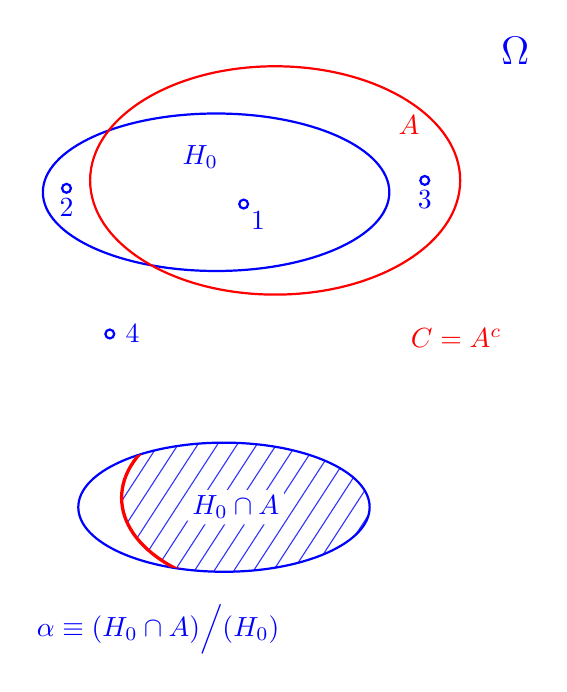
\begin{tikzpicture}[scale=1.0]
    % Espacio muestral Omega
    \node[blue, font=\Large] at (3.6, 2.6) {$\Omega$};

    % Conjunto H_0 (elipse azul) y conjunto A (elipse roja)
    \draw[blue, thick] (-0.2, 0.8) ellipse (2.2cm and 1.0cm);
    \node[blue] at (-0.4, 1.25) {$H_0$};

    \draw[red, thick] (0.55, 0.95) ellipse (2.35cm and 1.45cm);
    \node[red, font=\bfseries] at (2.25, 1.65) {$A$};

    % Puntos 1, 2, 3, 4 (los 4 escenarios)
    \draw[blue, thick] (0.15, 0.65) circle (1.6pt) node[below right=-1pt, blue] {$1$};
    \draw[blue, thick] (-2.1, 0.85) circle (1.6pt) node[below, blue] {$2$};
    \draw[blue, thick] (2.45, 0.95) circle (1.6pt) node[below, blue] {$3$};
    \draw[blue, thick] (-1.55, -1) circle (1.6pt) node[right=2pt, blue] {$4$};

    % Región crítica C = A^c
    \node[red, font=\bfseries] at (2.85, -1.05) {$C = A^c$};

    % Diagrama inferior: H_0 \cap A rayado diagonalmente con recorte exacto
    \begin{scope}[shift={(-0.1, -3.2)}]
      % Rayado diagonal recortado exactamente a la intersección de H_0 y A
      \begin{scope}
        \clip (0, 0) ellipse (1.85cm and 0.82cm);
        \clip (0.65, 0.12) ellipse (1.95cm and 1.18cm);
        \foreach \x in {-2.5, -2.25, ..., 2.5} {
          \draw[blue!80, thin] (\x, -1.0) -- (\x + 1.3, 1.0);
        }
      \end{scope}

      % Contorno completo de H_0 en azul
      \draw[blue, thick] (0, 0) ellipse (1.85cm and 0.82cm);

      % Arco rojo de frontera de A que corta a H_0 por la izquierda
      \begin{scope}
        \clip (0, 0) ellipse (1.85cm and 0.82cm);
        \draw[red, very thick] (0.65, 0.12) ellipse (1.95cm and 1.18cm);
      \end{scope}

      % Etiqueta H_0 \cap A sobre fondo blanco para legibilidad
      \node[blue, fill=white, inner sep=2pt, rounded corners=2pt] at (0.15, 0.0) {$H_0 \cap A$};
    \end{scope}

    % Fórmula inferior
    \node[blue, anchor=west] at (-2.6, -4.75)
      {$\alpha \equiv \Prob(H_0 \cap A)\Big/\Prob(H_0)$};
  \end{tikzpicture}
  \caption*{Figura 3. Los 4 escenarios posibles y errores de tipo I, II. Representación conjuntista de $H_0$, evidencia $A$, región crítica $C = A^c$ y probabilidad condicional $\alpha$.}
  \label{fig:h0-a-esquema}
\end{figure}


\section{Contraste de hipótesis sobre una proporción}

Cierto suceso tiene probabilidad $p$ desconocida y creemos que $p = p_0$. Queremos decidir si es cierto. Para ello repetimos $n$ veces el e.a.\ y contamos cuántas hay éxito, digamos $n_1 \le n$. Si $X_k \in \{0,1\}$ es la v.a.\ que marca si en la repetición $k$-ésima hubo éxito, tenemos $X_i \sim \operatorname{Bernoulli}(p)$ con $p$ desconocida.

La función de masa marginal y conjunta (verosimilitud) son
\[
  f_{X_1}(x) = p^x q^{1-x} = \begin{cases} p, & x=1, \\ q, & x=0; \end{cases} \qquad f(x_1, x_2, \dots, x_n; p) = p^{x_1 + \dots + x_n} q^{n - (x_1 + \dots + x_n)}.
\]
El MLE de $p$ es $\Theta = \overline{X}_n$, que es suficiente y minimal pues 
$$f(x_1, \dots, x_n; p) = p^{n\overline{x}_n}(1-p)^{n(1-\overline{x}_n)} \equiv h(\overline{x}_n; p)$$
por el TCL y el Teorema de De Moivre tenemos que
$$X_1 + \dots + X_n \sim \operatorname{Bin}(n,p) \approx \mathcal{N}(np, npq) \implies \Theta = \overline{X}_n \approx \mathcal{N}(p, pq/n)$$
Además $\overline{x}_n = n_1/n$. Bajo la hipótesis $p = p_0$, el $\alpha$-intervalo de confianza para $\overline{X}_n \approx \mathcal{N}(p_0, p_0 q_0 / n)$ es $(p_0 - \Sigma z,\, p_0 + \Sigma z)$, $\Sigma^2 = p_0 q_0 / n$. No rechazaremos si y solo si se cumple $\Theta(\omega) \in I_\Theta(p_0)$:
\[
  \overline{x}_n\equiv \frac{n_1}{n} \in (p_0 - \Sigma z,\, p_0 + \Sigma z) \quad \text{o bien} \quad n_1 \in (p_0 n - \Sigma n z,\, p_0 n + \Sigma n z).
\]

\begin{definicion}[76 --- $p$-valor]
Dada una muestra aleatoria $\vec{X}$ dependiente de un parámetro desconocido $\theta$, y un estadístico $\Theta_n = T(\vec{X})$ con regla de decisión ``rechazar $H_0$ si $T(\vec{X}(\omega)) \in F = (c, \infty)$'', observado $\vec{X}(\omega) = \vec{x}$ y $T(\vec{x}) = t$, el \emph{$p$-valor} es la probabilidad de obtener un resultado al menos tan extremo como el resultado realmente observado, bajo el supuesto de que $H_0$ es cierta. Si $\overline{F} = 1 - F$ es la cola:
\[
  p = \Prob\bigl(T(\vec{X}) \ge t \mid H_0\bigr) \equiv \overline{F}_{T(\vec{X})}(t) \quad \text{cuando } F = (c, \infty);
\]
\[
  p = \Prob\bigl(T(\vec{X}) \le t \mid H_0\bigr) \equiv F_{T(\vec{X})}(t) \quad \text{cuando } F = (-\infty, c).
\]
Mide la \underline{significancia estadística} del test: cuanto mayor sea $p$, más plausible hace la hipótesis $H_0$. 

Si el $p$-valor obtenido es mayor que el nivel de significación $1-\alpha$, no rechazaremos la hipótesis nula; en caso contrario, sí. 

El $p$-valor de un test es el nivel de significación más bajo con el que podemos rechazar $H_0$ para un resultado observado.
\end{definicion}

\noindent \textbf{Importante:} $\Prob(\text{observación} \mid \text{hipótesis}) \neq \Prob(\text{hipótesis} \mid \text{observación})$. Usar el valor $p$ como un ``puntaje'' de veracidad de $H_0$ es cometer la \emph{falacia de transposición condicional}.
\begin{figure}[htbp]
  \centering
  % --- Recuadro superior ---
  \fbox{\parbox{0.88\linewidth}{
    \vspace{0.35em}
    \noindent\textbf{Importante:}\\[0.5em]
    $\Prob(\text{observación} \mid \text{hipótesis}) \neq \Prob(\text{hipótesis} \mid \text{observación})$\\[0.5em]
    La probabilidad de observar un resultado dada una cierta hipótesis cierta \emph{no es equivalente} a la probabilidad de que una hipótesis sea cierta dado un resultado observado.\\[0.5em]
    Usar el valor $p$ como un ``puntaje'' es cometer un error lógico inmenso:\\
    \textbf{la falacia de transposición condicional.}
    \vspace{0.35em}
  }}

  \vspace{1.2em}

  % --- Diagrama TikZ del valor p ---
  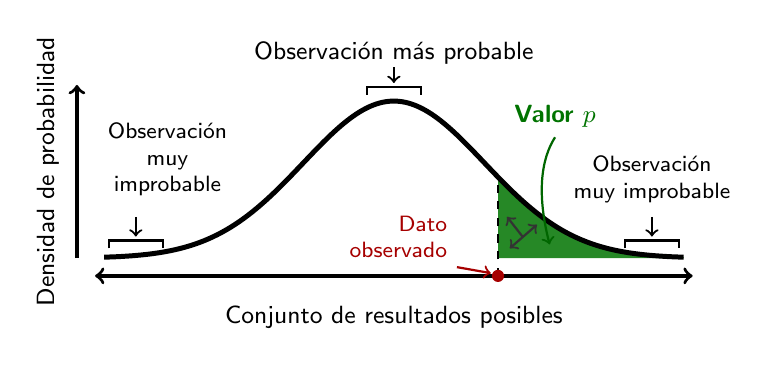
\begin{tikzpicture}[x=1.15cm, y=5cm]
    \def\gauss#1{exp(-0.5*(#1)^2)/sqrt(2*pi)}
    \def\xobs{1.15}

    % Área verde (Valor p) a la derecha del dato observado
    \fill[green!45!black, opacity=0.85, domain=\xobs:3.2, samples=90]
      (\xobs, 0) -- plot (\x, {\gauss{\x}}) -- (3.2, 0) -- cycle;

    % Eje horizontal con flechas en ambos extremos
    \draw[<->, very thick] (-3.3, -0.045) -- (3.3, -0.045)
      node[midway, below=7pt, font=\sffamily\small] {Conjunto de resultados posibles};

    % Eje vertical izquierdo con flecha y etiqueta girada
    \draw[->, very thick] (-3.5, 0) -- (-3.5, 0.44);
    \node[rotate=90, font=\sffamily\small] at (-3.82, 0.22) {Densidad de probabilidad};

    % Curva normal
    \draw[line width=1.8pt, domain=-3.2:3.2, samples=180] plot (\x, {\gauss{\x}});

    % Línea vertical discontinua en el dato observado
    \draw[dashed, thick] (\xobs, -0.045) -- (\xobs, {\gauss{\xobs}});

    % Punto rojo "Dato observado" y flecha indicadora
    \fill[red!65!black] (\xobs, -0.045) circle (2.2pt);
    \node[red!65!black, font=\sffamily\footnotesize, align=right] (dato) at (0.05, 0.055)
      {Dato\\observado};
    \draw[->, thick, red!65!black] (dato.south east) -- (1.07, -0.038);

    % Corchete y etiqueta superior: Observación más probable
    \draw[thick] (-0.30, 0.415) -- (-0.30, 0.435) -- (0.30, 0.435) -- (0.30, 0.415);
    \draw[->, thick] (0, 0.485) -- (0, 0.445);
    \node[font=\sffamily\small] at (0, 0.52) {Observación más probable};

    % Corchete izquierdo: Observación muy improbable
    \draw[thick] (-3.15, 0.025) -- (-3.15, 0.045) -- (-2.55, 0.045) -- (-2.55, 0.025);
    \draw[->, thick] (-2.85, 0.105) -- (-2.85, 0.055);
    \node[font=\sffamily\footnotesize, align=center] at (-2.5, 0.25)
      {Observación\\ muy \\improbable};

    % Corchete derecho: Observación muy improbable
    \draw[thick] (2.55, 0.025) -- (2.55, 0.045) -- (3.15, 0.045) -- (3.15, 0.025);
    \draw[->, thick] (2.85, 0.105) -- (2.85, 0.055);
    \node[font=\sffamily\footnotesize, align=center] at (2.85, 0.2)
      {Observación\\muy improbable};

    % Etiqueta "Valor p" y flechas hacia la región verde
    \node[green!45!black, font=\sffamily\bfseries\small] (vp) at (1.78, 0.36) {Valor $p$};
    \draw[->, thick, green!40!black] (vp.south) .. controls (1.62, 0.25) and (1.58, 0.16) .. (1.72, 0.035);
    \draw[<->, thick, black!80] (1.28, 0.025) -- (1.58, 0.085);
    \draw[->, thick, black!80] (1.42, 0.055) -- (1.25, 0.105);
  \end{tikzpicture}

  \vspace{0.7em}

  % --- Texto explicativo inferior ---
  \parbox{0.92\linewidth}{\centering\sffamily\small
    El \textcolor{green!45!black}{\textbf{valor $p$}} (área de color verde) es la probabilidad de que un valor observado sea igual o más extremo que un cierto valor, asumiendo que la hipótesis nula es cierta.
  }

  \caption*{Figura 4. Densidad de probabilidad de $\Theta$, quizá Gaussiana, y el $p$-valor.}
  \label{fig:densidad-valor-p}
\end{figure}\begin{figure}[htbp]
  \centering
  \begin{tikzpicture}[x=1.15cm, y=8cm]
    \def\gauss#1{exp(-0.5*(#1)^2)/sqrt(2*pi)}
    \def\xthr{1.45}
    \def\xobs{1.75}

    % Cuadrícula suave de fondo
    \draw[gray!12, very thin] (-3.5, 0) grid (3.4, 0.48);

    % Área verde (observed p-value statistical significance) a la derecha de \xobs
    \fill[green!60!black, opacity=0.88, domain=\xobs:3.2, samples=90]
      (\xobs, 0) -- plot (\x, {\gauss{\x}}) -- (3.2, 0) -- cycle;

    % Eje horizontal principal (gris) con marcas inferiores
    \draw[-{Latex[length=2.5mm]}, thick, gray!80] (-3.5, 0) -- (3.55, 0);
    \foreach \x in {-2.2, -1.1, 0, 1.1, 2.2} {
      \draw[gray!70, thin] (\x, 0) -- (\x, -0.012);
    }

    % Doble flecha inferior: Set of possible results
    \draw[{Latex[length=2.2mm]}-{Latex[length=2.2mm]}, thick, black] (-3.2, -0.042) -- (3.2, -0.042)
      node[midway, below=6pt, font=\sffamily\slshape\small, gray!80] {Set of possible results};

    % Eje vertical izquierdo: Probability of observation
    \draw[-{Latex[length=2.5mm]}, thick, gray!80] (-3.5, 0) -- (-3.5, 0.48);
    \node[rotate=90, font=\sffamily\slshape\small, gray!80] at (-3.85, 0.24) {Probability of observation};

    % Curva normal verde
    \draw[line width=1.4pt, green!65!black, domain=-3.2:3.2, samples=180] plot (\x, {\gauss{\x}});

    % Etiqueta superior: true value under the null hypothesis and most likely observation
    \node[green!65!black, font=\sffamily\bfseries\slshape\footnotesize, align=center, above] (top) at (0, 0.435)
      {true value under the null\\hypothesis and most likely observation};
    \draw[-{Latex[length=1.8mm]}, thick, green!65!black] (top.south) -- (0, 0.405);

    % Línea vertical discontinua del umbral (95% statistical significance threshold)
    \draw[dashed, thick, gray!80] (\xthr, 0.008) -- (\xthr, 0.27);
        \node[gray!80, font=\sffamily\bfseries\slshape\footnotesize, align=left, anchor=west] (thr) at (1.6, 0.35)
          {95\% statistical\\significance threshold};
        \draw[-{Latex[length=1.8mm]}, thick, gray!80] (thr.west) -- (\xthr + 0.02, 0.21);
    % Punto naranja: observed result (value)
    \fill[orange!90!black] (\xobs, 0.008) circle (3.2pt);
    \node[orange!90!black, font=\sffamily\bfseries\slshape\footnotesize, align=right, anchor=east] (obs) at (1.32, 0.05)
      {observed\\result (value)};
    \draw[-{Latex[length=1.8mm]}, thick, orange!90!black] (obs.east) -- (\xobs - 0.14, 0.015);

    % Etiqueta de p-valor a la derecha (desplazada hacia abajo para no tocar el umbral)
    \node[green!65!black, font=\sffamily\bfseries\slshape\footnotesize, align=left, anchor=west] (pval) at (1.98, 0.22)
      {observed $p$-value\\statistical significance};
    \draw[-{Latex[length=1.8mm]}, thick, green!65!black] (pval.south west) -- (2.02, 0.038);

    % Segmentos con topes: very unlikely observations (izquierda y derecha)
    \draw[thick, black!85] (-3.25, 0.016) -- (-3.25, 0.026) (-3.25, 0.021) -- (-2.25, 0.021) (-2.25, 0.016) -- (-2.25, 0.026);
    \node[font=\sffamily\bfseries\slshape\scriptsize, align=center, above] at (-2.75, 0.028)
      {very unlikely\\observations};

    \draw[thick, black!85] (2.25, 0.016) -- (2.25, 0.026) (2.25, 0.021) -- (3.25, 0.021) (3.25, 0.016) -- (3.25, 0.026);
    \node[font=\sffamily\bfseries\slshape\scriptsize, align=center, above] at (2.75, 0.028)
      {very unlikely\\observations};
  \end{tikzpicture}
  \caption*{Figura 5. Densidad de probabilidad de $\Theta$, quizá Gaussiana, y el $p$-valor.}
  \label{fig:densidad-valor-p2}
\end{figure}
\begin{figure}[htbp]
  \centering
  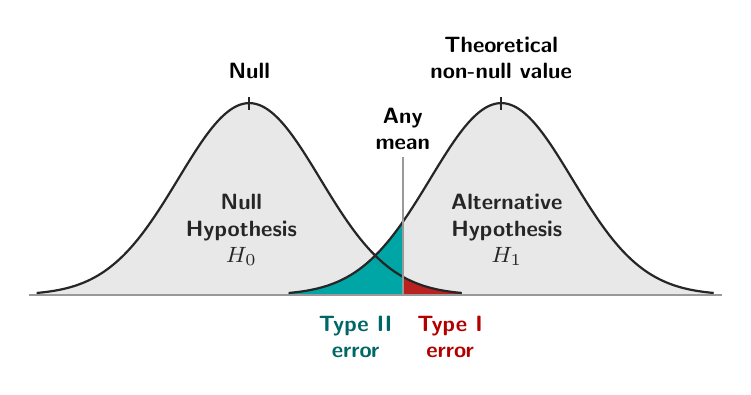
\begin{tikzpicture}[x=1.0cm, y=5.5cm]
    % Dos curvas normales: H_0 centrada en -1.6 y H_1 centrada en +1.6
    \def\gnull#1{exp(-0.5*((#1 + 1.6)/0.9)^2)/(0.9*sqrt(2*pi))}
    \def\galt#1{exp(-0.5*((#1 - 1.6)/0.9)^2)/(0.9*sqrt(2*pi))}
    \def\xcut{0.35}

    % Relleno gris claro bajo ambas curvas
    \fill[gray!18, domain=-4.3:0.35, samples=120]
      (-4.3, 0) -- plot (\x, {\gnull{\x}}) -- (0.35, 0) -- cycle;
    \fill[gray!18, domain=-1.1:4.3, samples=120]
      (-1.1, 0) -- plot (\x, {\galt{\x}}) -- (4.3, 0) -- cycle;

    % Área Type II error (azul verdoso): bajo H_1 a la izquierda del corte
    \fill[teal!70!cyan, domain=-1.1:\xcut, samples=80]
      (-1.1, 0) -- plot (\x, {\galt{\x}}) -- (\xcut, 0) -- cycle;

    % Área Type I error (rojo): bajo H_0 a la derecha del corte
    \fill[red!70!black, opacity=0.85, domain=\xcut:1.1, samples=80]
      (\xcut, 0) -- plot (\x, {\gnull{\x}}) -- (1.1, 0) -- cycle;

    % Eje horizontal base
    \draw[thick, gray!80] (-4.4, 0) -- (4.4, 0);

    % Contornos de las dos curvas
    \draw[thick, black!85, domain=-4.3:1.1, samples=160] plot (\x, {\gnull{\x}});
    \draw[thick, black!85, domain=-1.1:4.3, samples=160] plot (\x, {\galt{\x}});

    % Marcas en las medias y línea vertical en el corte ("Any mean")
    \draw[thick, black!85] (-1.6, {\gnull{-1.6} - 0.015}) -- (-1.6, {\gnull{-1.6} + 0.015});
    \node[font=\sffamily\bfseries\footnotesize, above=3pt] at (-1.6, {\gnull{-1.6} + 0.015}) {Null};

    \draw[thick, black!85] (1.6, {\galt{1.6} - 0.015}) -- (1.6, {\galt{1.6} + 0.015});
    \node[font=\sffamily\bfseries\footnotesize, align=center, above=3pt] at (1.6, {\galt{1.6} + 0.015})
      {Theoretical\\non-null value};

    \draw[thick, gray!80] (\xcut, 0) -- (\xcut, 0.32);
    \node[font=\sffamily\bfseries\footnotesize, align=center, above=2pt] at (\xcut, 0.3)
      {Any\\mean};

    % Etiquetas interiores de las hipótesis
    \node[font=\sffamily\bfseries\footnotesize, align=center, black!85] at (-1.7, 0.15)
      {Null\\Hypothesis\\$H_0$};
    \node[font=\sffamily\bfseries\footnotesize, align=center, black!85] at (1.67, 0.15)
      {Alternative\\Hypothesis\\$H_1$};

    % Etiquetas inferiores: Type II error y Type I error
    \node[teal!80!black, font=\sffamily\bfseries\footnotesize, align=center, below=4pt] at (-0.25, 0)
      {Type II\\error};
    \node[red!70!black, font=\sffamily\bfseries\footnotesize, align=center, below=4pt] at (0.95, 0)
      {Type I\\error};
  \end{tikzpicture}
  \caption*{Figura 6. Errores de tipo I y tipo II en contraste simple/simple.}
  \label{fig:errores-tipo-i-ii}
\end{figure}















\section{Otros tests: problema de contraste unilateral de medias}

Dada una muestra aleatoria $X_1, \dots, X_n$ dependiente de un parámetro desconocido $\theta$, en un test de hipótesis podemos particionar el espacio de parámetros $\theta \in \Xi = \Xi_0 \cup \Xi_1$. Tendremos que determinar:
\begin{enumerate}
  \item Hipótesis nula: $H_0 : \theta \in \Xi_0$ versus $H_1 : \theta \in \Xi_1$.
  \item Estimador de contraste $\Theta$.
  \item Regla de decisión y región de rechazo $F \subset \R$: normalmente la rddes ``Rechazar $H_0$ si $\Theta(\omega) \in F$''.
\end{enumerate}

\begin{definicion}[77]
Dada una muestra aleatoria $X_1, \dots, X_n$ dependiente de un parámetro desconocido $\theta$, un estadístico $\Theta_n = T(X_1, \dots, X_n)$, un nivel $\alpha \in \R$ y $F_\alpha \subset \R$ un subconjunto de la recta real. Supongamos que la regla de decisión es de la forma \begin{center}``Rechazar $H_0$ al nivel $\alpha$ si $T(\vec{X}(\omega)) \in F_\alpha$''\end{center} En el caso bilateral será $\Theta(\omega) \notin I_\Theta(\theta_0)$, con $\alpha = \Prob(\Theta \in I_\Theta(\theta_0) \mid \theta = \theta_0)$ la probabilidad de no rechazo. Entonces:
\begin{enumerate}
  \item $T(\vec{X})$ es el estadístico del test;
  \item $F \subset \R$ es la región de rechazo de la prueba;
  \item El conjunto $S_1 \coloneqq \{\vec{x} : T(\vec{x}) \in F\} \subset \R^n$ es la región crítica en el espacio muestral;
  \item El conjunto $C \coloneqq \vec{X}^{-1}(S_1) \coloneqq \{\omega : T(\vec{X}(\omega)) \in F\} \subset \Omega$ es la región crítica en $\Omega$. Nota: $C^c = A = \{\omega : \Theta(\omega) \in I_\Theta(\theta_0)\}$.
\end{enumerate}
\end{definicion}

\begin{definicion}[78 --- \underline{Tipos básicos de test}] \, 
\begin{enumerate}
  \item Contraste bilateral: $\Xi_0 = \{\theta_0\}$; $\Xi_1 = \R \setminus \{\theta_0\}$.
  \item Contraste unilateral superior: $\Xi_0 = \{\theta_0\}$; $\Xi_1 = \{\theta > \theta_0\} = (\theta_0, \infty)$.
  \item Contraste unilateral inferior: $\Xi_0 = \{\theta_0\}$; $\Xi_1 = \{\theta < \theta_0\} = (-\infty, \theta_0)$.
  \item Simple / Simple o de dos puntos: $\Xi_0 = \{\theta_0\}$; $\Xi_1 = \{\theta_1\}$.
\end{enumerate}
\end{definicion}

\begin{definicion}[79 --- \underline{Metodología de trabajo}]
Se busca minimizar simultáneamente los dos tipos de errores. Como esto en general no es posible, elegimos un valor crítico $\alpha$ tan cercano a $1$ como queramos y buscamos, entre todas las regiones de rechazo de tamaño $1-\alpha$, aquella que minimice la probabilidad de cometer un error de tipo II:
\begin{enumerate}
  \item Decidir el tipo de test necesario.
  \item En test de dos puntos, construir un test de \underline{máxima potencia} a nivel $\alpha$, es decir, definir la región crítica $C$, o $F$, de modo que satisfaga:
  \begin{enumerate}[label=(\alph*)]
    \item $\Prob(\text{error de tipo I}) = \Prob(\Theta \in F \mid \theta = \theta_0) = 1 - \alpha$;
    \item Para este valor $\alpha$ deseado, minimice además $\Prob(\text{error de tipo II}) = 1 - \beta$;
    \item Para poder satisfacer simultáneamente ambas condiciones necesitamos tomar $F$ generales, pues si tomamos el complementario del i.c.\ satisfacemos (a) pero no necesariamente (b).
  \end{enumerate}
\end{enumerate}

\noindent \textbf{Algunas regiones de rechazo:}
\begin{enumerate}
  \item Contraste bilateral $H_0 : \theta = \theta_0$ versus $H_1 : \theta \neq \theta_0$: la región de rechazo es el conjunto complementario del i.c.\ de nivel $\alpha$: $F = (a_-, a_+)^c$, $a_\pm = F_\Theta^{-1}((1\pm\alpha)/2)$.
  \item Contraste unilateral inferior $H_0 : \theta = \theta_0$ versus $H_1 : \theta < \theta_0$: la región de rechazo es $F = (-\infty, F_\Theta^{-1}(1-\alpha))$.
  \item Contraste unilateral superior $H_0 : \theta = \theta_0$ versus $H_1 : \theta > \theta_0$: la región de rechazo es $F = (F_\Theta^{-1}(\alpha), \infty)$.
  \item Simple versus simple: $H_0 = \{\theta = \theta_0\}$, hipótesis alternativa $H_1 = \{\theta = \theta_1\}$.
\end{enumerate}
\end{definicion}

\subsection{Pruebas de razón de verosimilitudes}

La función de verosimilitud tiende a ser máxima cerca del valor verdadero de $\theta$. De hecho, esta es la razón por la que la estimación de máxima verosimilitud funciona bien.

\subsection{Contraste de hipótesis simple versus simple}

Se denomina así a los tests donde la hipótesis nula es $H_0 = \{\theta = \theta_0\}$ y la hipótesis alternativa es $H_1 = \{\theta = \theta_1\}$:
\begin{enumerate}
  \item No rechazar $H_0$ (ha ocurrido $A$) siendo $H_0$ correcta: $\Prob(\text{escenario 1}) = \Prob(\Theta \notin C(\theta_0) \mid \theta = \theta_0) = \alpha$.
  \item Rechazar $H_0$ siendo $H_0$ correcta: $\Prob(\text{error de tipo I}) = \Prob(\Theta \in C(\theta_0) \mid \theta = \theta_0) = 1 - \alpha$.
  \item Aceptar / no rechazar $H_0$ siendo $H_0$ falsa: $\Prob(\text{error de tipo II}) = \Prob(\Theta \notin C(\theta_0) \mid \theta = \theta_1) \equiv 1 - \beta$.
  \item Rechazar $H_0$ siendo $H_0$ falsa: $\Prob(\text{escenario 4}) = \Prob(\Theta \in C(\theta_0) \mid \theta = \theta_1) \equiv \beta$ (potencia del test).
\end{enumerate}

\begin{teorema}[30 --- Lema de Neyman-Pearson]
Dado un test simple versus simple, y fijado el nivel $\alpha$, en un test de máxima potencia a nivel $\alpha$ la región crítica de mayor potencia para el test es $C_k \subset \Omega$ definida por $\Prob(C_k \mid H_0) = 1 - \alpha$ y
\[
  C_k = \bigl\{\omega : Q(\vec{X}(\omega)) < k\bigr\} \subset \Omega, \qquad \text{donde } Q(\vec{X}) \equiv \frac{f_{\vec{X}}(\vec{X}; \theta_0)}{f_{\vec{X}}(\vec{X}; \theta_1)}.
\]
Regla de decisión: rechazaremos $H_0$ o no dependiendo de que la razón de verosimilitudes satisfaga $\omega \in C_k$ o no. Alternativamente, si la muestra $\vec{x}$ satisface $$\vec{x} \in S \coloneqq \{\vec{x} : Q(\vec{x}) < k\} \subset \R^n \quad (\text{Nota}: C = \vec{X}^{-1}(S) \subset \Omega)$$
La constante $k$ queda fijada por $\Prob(C_k \mid H_0) = 1 - \alpha$. El test de máxima potencia puede no existir o no ser único.
\end{teorema}

\begin{corolario}[6]
Si además el test se basa en un estadístico suficiente $T(\vec{X})$ con factorización $f_{\vec{X}}(\vec{x};\theta) = g(T(\vec{x});\theta)h(\vec{x})$, rechazaremos $H_0$ si y solo si la muestra satisface, con:
\[
  T(\vec{x}) = t; \quad \frac{g(t; \theta_0)}{g(t; \theta_1)} < k.
\]
\textbf{Metodología:}
\begin{enumerate}
  \item Elegir un estadístico suficiente $T(\vec{x})$.
  \item Sea $\Psi(t; \theta_0, \theta_1) \equiv \dfrac{g(t; \theta_0)}{g(t; \theta_1)}$. Entonces, en el caso más favorable, resolvemos la ec.
  \[
    t \mapsto \Psi(t; \theta_0, \theta_1) < k \implies t > \Psi^{-1}(t; \theta_0, \theta_1), \infty) \equiv c \implies C = \{\vec{X} : T(\vec{X}) < c\}
  \]
  y obtener la región crítica
  \[
    C = \{\vec{x} : T(\vec{x}) \in F \equiv (-\infty, \Psi^{-1}(t; \theta_0, \theta_1))\}
  \]
  Además la constante $k$ debe satisfacer $\Prob\!\left(\frac{g(T(\vec{X}); \theta_0)}{g(T(\vec{X}); \theta_1)} < k\right) = 1 - \alpha$.

  \item Calcular probabilidad de error de tipo II
  \[
    \Prob(\omega \notin C \mid \theta = \theta_1) = \Prob(\vec{X}) > c(\alpha) \mid \theta = \theta_1)
  \].
\end{enumerate}
\end{corolario}
\textcolor{blue}{
\section{Problemas más generales}
Otros problemas usuales se obtienen con $\Xi_0$ y $\Xi_1 = \Xi_0^c$ dos regiones del espacio de parámetros. Con generalidad queremos probar $\{H_0 : \theta \in \Xi_0\}$ y $\{H_1 : \theta \in \Xi_1\}$.
\begin{definicion}[80]
Dada la hipótesis nula $H_0 = \{\theta = \theta_0\}$, con nivel $\alpha$, teníamos $\Theta \coloneqq T(X_1, \dots, X_n)$, estimador insesgado consistente de $\theta$, y $I_\Theta(\theta_0)$ el intervalo de confianza bajo la hipótesis $H_0$. La \emph{función potencia} del test es
\[
  \pi(t) = \Prob\bigl(\Theta \notin I_\Theta(\theta_0) \mid \theta = t\bigr).
\]
En particular $\pi(\theta_0) = 1 - \alpha$. Si $\theta \in \Xi_0$, $\pi(t)$ es la probabilidad de cometer un error de tipo I; si $\theta \in \Xi_1$, $1 - \pi(t)$ es la probabilidad de cometer un error de tipo II. Una buena función de potencia debe satisfacer $\pi(\theta) \approx 0$ si $\theta \in \Xi_0$ y $\pi(\theta) \approx 1$ si $\theta \in \Xi_1$. Para obtener un buen balance procedemos como sigue:
\begin{enumerate}
  \item Fijar un límite para la probabilidad de cometer el error de tipo I: $\pi(\theta) \le 1 - \alpha$ para $\theta \in \Xi_0$ (nivel de significación de la prueba).
  \item Excluir todos aquellos tests con regiones críticas que no respeten el límite para el error de tipo I. Entre los que lo respeten, seleccionar aquel que minimice el error de tipo II, es decir, maximice $\pi(\theta)$ si $\theta \in \Xi_1$.
  \item Otra posibilidad: minimizar una combinación lineal de las diferentes probabilidades de error.
\end{enumerate}
\end{definicion}
\begin{definicion}[81 --- Pruebas de razón de verosimilitudes]
Sea $f_{\vec{X}}(\vec{x};\theta)$ la verosimilitud y
\[
  s(\vec{x}) \coloneqq \sup_{\theta \in \Xi_0} f_{\vec{X}}(\vec{x};\theta); \qquad S(\vec{x}) \coloneqq \sup_{\theta \in \Xi} f_{\vec{X}}(\vec{x};\theta); \qquad \Gamma(\vec{x}) = \frac{s(\vec{x})}{S(\vec{x})}.
\]
Regla de decisión: elegido un valor $k$, ``no rechazar la hipótesis'' si y solo si la observación $\vec{x}_0$ satisface $\Gamma(\vec{x}_0) > k$.
\end{definicion}
\begin{proposicion}[91 --- Pruebas de razón de verosimilitudes para estadísticos suficientes]
Supongamos que $T(\vec{x})$ es un estadístico suficiente. Entonces $\Gamma(\vec{x})$ es constante en la clase de equivalencia $C_t = \{\vec{x} : T(\vec{x}) = t\}$ de valor
\[
  \Gamma(\vec{x}) \equiv \Gamma(t) = \frac{\sup_{\theta \in \Xi_0} g(t;\theta)}{\sup_{\theta \in \Xi} g(t;\theta)},
\]
y la regla de decisión es idéntica para todas las observaciones en la misma clase de equivalencia.
\end{proposicion}
\begin{proof}
Si $T(\vec{x})$ es un estadístico suficiente, por la factorización de Fisher-Neyman $f_{\vec{X}}(\vec{x};\theta) = g(T(\vec{x});\theta)\,h(\vec{x})$, de donde
\[
  \Gamma(\vec{x}) = \frac{\sup_{\theta \in \Xi_0} f_{\vec{X}}(\vec{x};\theta)}{\sup_{\theta \in \Xi} f_{\vec{X}}(\vec{x};\theta)} = \frac{h(\vec{x})}{h(\vec{x})}\cdot\frac{\sup_{\theta \in \Xi_0} g(T(\vec{x});\theta)}{\sup_{\theta \in \Xi} g(T(\vec{x});\theta)} = \frac{\sup_{\theta \in \Xi_0} g(t;\theta)}{\sup_{\theta \in \Xi} g(t;\theta)}. \qedhere
\]
\end{proof}
Regla de decisi\'on: Elegido un valor $k\ll$, ``no rechazar la hip\'otesis si y solo si la observaci\'on $\vec{x}_0$ satisface $\Gamma(\vec{x}_0) > k$.}

% =========================================================================
\section{Tipos de test más frecuentes}

Los casos 1 a 6 son todos variaciones sobre un mismo tema. Caso 1: distribución binomial aproximada a normal. Casos 2--6: distribución normal. Caso 7 es diferente.
\begin{enumerate}
  \item \textbf{Contraste bi(uni)lateral de proporciones:} $H_0 : p = p_0$ versus $H_1 : p \neq p_0$ ($p > p_0$, $p < p_0$). Pivote: media muestral tipificada.
  \item \textbf{Contraste bi(uni)lateral de media con varianza conocida:} $H_0 : \mu = \mu_0$ versus $H_1 : \mu \neq \mu_0$ ($\mu > \mu_0$, $\mu < \mu_0$). Pivote: media muestral tipificada.
  \item \textbf{Contraste bi(uni)lateral de media con varianza desconocida:} Pivote $t$-Student.
  \item \textbf{Contraste bi(uni)lateral de media de la diferencia de poblaciones independientes con varianza conocida:} Reducir al anterior (2) con $\mu_0 = 0$ bajo $H_0$ y varianza la suma $\sigma_1^2 + \sigma_2^2$.
  \item \textbf{Contraste bi(uni)lateral de media de la diferencia de poblaciones independientes con varianza desconocida:} Reducir al anterior (3) con $\mu_0 = 0$ bajo $H_0$, y varianza combinada / $t$-Student.
  \item \textbf{Contraste bi(uni)lateral de media de la diferencia de poblaciones dependientes anidadas con varianza desconocida:} Similar, reducir a (3) con $\mu_0 = 0$ bajo $H_0$ y calcular media y varianza muestrales para la diferencia.
  \item \textbf{Contraste a dos puntos:} $H_0 : \mu = \mu_0$ versus $H_1 : \mu = \mu_1$. Usar el Lema de Neyman-Pearson.
\end{enumerate}
\noindent\underline{Tipos de test más frecuentes}

\[
  \resizebox{0.98\linewidth}{!}{$
  \left\{
  \begin{array}{l}
    \text{Contraste bi(uni)lateral de media con varianza }
    \left\{
    \begin{array}{l}
      \text{conocida} \\
      \text{desconocida} \\
      \text{función de la media (proporciones)}
    \end{array}
    \right. \\[1.4em]
    \text{Contraste bi(uni)lateral de media de la diferencia de poblaciones independientes con varianza }
    \left\{
    \begin{array}{l}
      \text{conocida} \\
      \text{desconocida}
    \end{array}
    \right. \\[1.1em]
    \text{Contraste ``\hspace{6.7cm}'' de poblaciones dependientes anidadas con varianza desconocida.} \\[0.4em]
    \text{Contraste a dos puntos } H_0 : \mu = \mu_0,\; H_1 : \mu = \mu_1.
  \end{array}
  \right.
  $}
\]


% =========================================================================
\section{Problemas}

\begin{enumerate}
  \item \textbf{Se ha jugado $1000$ veces a la ruleta y han salido $464$ veces rojo y $536$ negro. Decidir a un nivel $\alpha = 0{,}95$ si la ruleta es justa o está manipulada.}

  \smallskip
  \noindent\emph{Solución:} Es un problema de contraste \underline{bilateral} de proporciones. Bajo la hipótesis de ruleta justa, $H_0 : p = 0{,}5$, y el intervalo de confianza para el número de rojos es $(470,\, 530)$ (Problema 1 anterior). Como $464 \notin (470,\, 530)$, debemos rechazar $H_0$, admitir que el
  croupier está haciendo trampa.

  \item \textbf{Una empresa fabrica clips de plástico y el proceso de fabricación debe ajustarse si la probabilidad de que un clip sea defectuoso supera el $10\%$. Para investigar si es necesario un ajuste, se comprueban $500$ clips seleccionados al azar y $55$ de ellos resultan defectuosos. Probar al nivel del $95\%$ si es necesario el ajuste.}
chal
  \smallskip
  \noindent\emph{Solución:} Es un problema de contraste \underline{unilateral de proporciones}. Las hipótesis son $H_0 : p = 0.1$ frente a $H_1 : p > 0.1$ y el test de hipótesis requiere un $\alpha$ intervalo de confianza $I_\Theta(\theta_0) \equiv (c, \infty)$
  \[
    \Prob(\overline{X}_n \geq a_+ \mid p = 0.1) = \alpha
  \]
  Bajo $H_0$ es
  \[
    \overline{X}_n \sim \mathcal N\left(p_0, \sqrt{p_0 q_0 / n}\right) = \mathcal N\left(0.1, \sqrt{0.09 / 500}\right); \quad P \coloneqq \frac{\overline{X}_n - 0.1}{\sqrt{0.09 / 500}} \sim \mathcal N(0, 1)
  \]
  \begin{enumerate}[label=(\alph*)]
    \item $P_n \geq c \iff \overline{X}_n \geq p_0 + c\sqrt{p_0 q_0 / n}$
    \item Elección de $c$
    \[
      \Prob(P_n \geq c \mid H_0) = 1 - \alpha \iff \Phi(c) = 0.95 \implies c = \Phi^{-1}(\alpha) = 1.64
    \]
    \item Regla de decisión: Rechazaremos si $P_n(\omega) \in F \coloneqq (c, \infty)$
  \end{enumerate}
  Aquí no rechazamos pues
  \[
    \overline{X}_n(\omega) = 0.11, \quad P(\omega) = 0.75 < 1.64
  \]
  El $p$-valor es
  \[
    p = \Prob(P \geq P(\omega) \mid H_0) = 1 - \Phi(0.75) = 0.23 \gg 0.05
  \]

  \item \textbf{$X =$ ``coeficiente intelectual de la población'' se distribuye normalmente con una media de $100$ y una desviación típica de $15$. Un nuevo método pedagógico afirma que consigue elevarlo después de su uso durante $12$ meses. Para evaluar el método, se ha probado con un grupo de ocho alumnos que arroja los resultados $X = 90, 92, 97, 114, 115, 120, 125, 127$. Decidir si puede asumirse que efectivamente el método funciona al nivel de confianza del $95\%$. Calcular el $p$-valor.}

  \smallskip
  \noindent\emph{Solución:}
  
  \noindent\underline{Contraste unilateral superior de medias en población $N(\mu, \sigma^2)$ con varianza conocida} con $H_0 : \mu = 100$, $H_1 : \mu > 100$.

  Tomamos el estimador $\Theta = \overline{X}_n$, $\alpha = 0.95$ (con $Q = 1.66$, $\overline{x}_n = 110$). Suponiendo que (hipótesis nula) $H_0 : X \sim N(100, 225)$ (el método no funciona) y exploramos la condición $1 - \alpha = \Prob(\overline{X}_n \geq a)$. Tenemos
  \[
    1 - \alpha = \Prob(\overline{X}_n \geq a) \iff 1 - \alpha = \Prob(N \geq (a - \mu)/\Sigma) = 1 - \Phi((a - \mu)/\Sigma)
  \]
  \[
    \iff \alpha = \Phi((a - \mu)/\Sigma) \iff a = \mu + \frac{\sigma}{\sqrt{n}} Q_\alpha
  \]
  Regla de decisión: No rechazar $H_0 \iff \overline{x}_n < \mu + \frac{\sigma}{\sqrt{n}} Q_\alpha \equiv a$.

  Las regiones de rechazo son
  \[
    F = (a, \infty); \quad S_1 \coloneqq \{\vec{x} : (x_1 + \dots + x_n > na\} \in \mathbb{R}^n; \quad C \coloneqq \{\omega : \overline{X}_n(\omega) > a\} \in \Omega
  \]
  Bajo la hipótesis nula $\mu = 100$ el valor obtenido
  \[
    t \equiv \overline{x}_n = 110; \quad \mu = 100; \quad Q_\alpha = 1.65; \quad \frac{\sigma}{\sqrt{n}} Q_\alpha = \frac{15}{\sqrt{8}} \times 1.65 = 8.75; \implies
  \]
  \[
    110 > \mu + \frac{\sigma}{\sqrt{n}} Q_\alpha = 108.75
  \]
  luego al nivel de seguridad del $95\%$ debemos rechazar $H_0$ y aceptar $H_1$ (el método sí funciona).

  El $p$-valor se calcula como
  \[
    p \coloneqq \Prob(\overline{X}_n \geq 110) = \Prob(N \geq (t - \mu)/\Sigma) = \Prob(N \geq 10 \times \sqrt{8}/15) = \Prob(N \geq 1.88) = 0.03
  \]
  bajo $H_0 : \mu = \mu_0$.

  \item \textbf{Un tratamiento afirma ser capaz de bajar el nivel de colesterol. Para probarlo se toma una muestra de dos poblaciones ambas $\mathcal{N}(\mu, \sigma^2)$ con medias desconocidas y varianzas conocidas donde una sí ha seguido el tratamiento y la otra no. Construir la regla de decisión para $H_0$: el tratamiento es un placebo versus $H_1 : H_0^c$ (bilateral).}

  \smallskip
  \noindent\emph{Solución:} \noindent\underline{Contraste bilateral de media de la diferencia con varianza conocida.}

  Si llamamos $X_1 \sim N(\mu_1, \sigma^2)$ ($X_2 \sim \mathcal N(\mu_2, \sigma^2)$) la población que sí (no) ha seguido el tratamiento, tenemos que son poblaciones \underline{independientes}, luego $Y \equiv X_1 - X_2 \sim \mathcal N(\mu_1 - \mu_2, 2\sigma^2)$.

  Las hipótesis a contrastar son ($\mu \equiv \mu_1 - \mu_2$)
  \begin{align*}
    H_0 &= \text{``el tratamiento es un placebo''} \iff \mu_1 - \mu_2 = 0; \quad X_1 - X_2 \sim \mathcal N(0, 2\sigma^2) \\
    H_1 &= \text{``el tratamiento no es un placebo''} \iff \mu \neq 0
  \end{align*}
  Usa el pivote
  \[
    P \coloneqq \frac{\overline{Y}}{\sqrt{2n}\sigma} \sim \mathcal N(0, 1)
  \]
  Rechazaremos si bajo $H_0$ es
  \[
    \overline{x}_1 - \overline{x}_2 \notin \bigl(-\sqrt{2n}\,a,\, \sqrt{2n}\,a\bigr),
  \]
  pues
  \[
    \Prob(|P_n| \leq a) = \alpha \implies a = \Phi^{-1}\bigl((1 + \alpha)/2\bigr)
  \]

  \item \textbf{Mismo problema cuando se trata de una misma población medida antes y después del tratamiento (datos apareados/anidados).}

  \smallskip
  \noindent\emph{Solución:} Construir la regla de decisión para $H_0:$ el tratamiento es un placebo versus $H_1 : H_0^c$ (bilateral).
  Si, por el contrario, $X_1 \sim \mathcal N(\mu_1, \sigma^2)$ ($X_2 \sim \mathcal N(\mu_2, \sigma^2)$) describen la población después (antes) de haber seguido el tratamiento, tenemos que obviamente $\vec{X}_1, \vec{X}_2$ no son poblaciones \underline{independientes}; pero (es la hip.\ del modelo lineal) $X_2 = X_1 + Y$ donde el ``residual $Y$ es indep.\ de $X_1$''. Luego $Y \equiv X_1 - X_2 \sim N(\mu_1 - \mu_2, 2\sigma_{X_1 - X_2}^2)$, donde $\sigma_{X_1 - X_2}$ la podemos calcular a través de los datos o bien usando la fórmula de varianza de una suma (ver lección 3, )
  \[
    \Var(X_1 - X_2) = \Var(X_1) + \Var(X_2) - 2\Cov(X_1, X_2) \leq \Var(X_1) + \Var(X_2)
  \]
  Lo demás queda igual.

  \item \textbf{Dada una población $\mathcal{N}(\mu, \sigma^2)$ con media y varianza desconocidas, construir la regla de decisión para $H_0 : \mu = \mu_0$ versus $H_1 : \mu > \mu_0$ (unilateral).}

  \smallskip
  \noindent\emph{Solución:} La distribución $t_n$ de Student con $n$ grados de libertad tiene densidad de probabilidad
  \[
    t_n \sim f(t) = k\left(1 + \frac{t^2}{n}\right)^{-(n+1)/2}, \quad k \equiv \frac{\Gamma\left(\frac{n+1}{2}\right)}{\sqrt{\pi n}\,\Gamma\left(\frac{n}{2}\right)}
  \]
  donde $\Gamma$ es la función gamma. El teorema de Fisher afirma $\overline{X}_n \perp S_n^2$. Además
  \[
    \overline{X}_n \sim N(\mu, \sigma^2/n) \perp \frac{n}{\sigma^2} S_n^2 \sim \chi^2_{n-1} \implies
  \]
  se obtiene como corolario que
  \[
    P_n := \sqrt{n-1}\,\frac{\overline{X}_n - \mu}{S_n} \sim t_{n-1}; \implies
  \]
  es un pivote y exploramos la condición
  \[
    1 - \alpha = \Prob(P \geq a) \iff a = \bar{F}_{t_{n-1}}^{-1}(1 - \alpha) = F_{t_{n-1}}^{-1}(\alpha)
  \]
  la región de rechazo es $F = \bigl(F_{t_{n-1}}^{-1}(\alpha), \infty\bigr)$.

  La condición de rechazo es $P_n(\omega) \in F$:
  \[
    \text{alternativamente } \sqrt{n-1}\,\frac{\overline{X}_n(\omega) - \mu}{S_n(\omega)} > F_{t_{n-1}}^{-1}(\alpha) \iff
  \]
  \[
    \overline{x}_n > \mu + \frac{S_n(\omega)}{\sqrt{n-1}}\,F_{t_{n-1}}^{-1}(\alpha)
  \]
  mientras que en el caso donde $\sigma$ es conocida la región de rechazo es
  \[
    \overline{x}_n > \mu + \frac{\sigma}{\sqrt{n}}\,\Phi^{-1}(\alpha)
  \]
  El $p$-nivel es bajo $H_0$
  \[
    p := \Prob(\overline{X}_n \geq \overline{X}_n(\omega) \mid \mu = \mu_0) = \Prob(P_n \geq P_n(\omega)) = \bar{F}_{t_{n-1}}(P_n(\omega))
  \]
  donde $P_n(\omega)$ es el valor observado para $P_n$.
  \item \textbf{Demostrar que en un contraste unilateral superior la Regla de decisión para $H_0$ es: rechazar si el valor observado del estadístico $T(\vec{x})$ satisface}
    \begin{enumerate}[label=(\alph*)]
      \item $t := T(\vec{x}) \geq Q_\alpha$
      \item o, $p = \Prob(T(\vec{X}) \geq t \mid H_0) \leq 1 - \alpha$,
    \end{enumerate}
    \textbf{Concluir que el $p$-valor es el mayor valor de $\alpha$ a partir del cual rechazamos $H_0$ con los datos observados.}

    \item \textbf{Calcular la región crítica para simple/simple con $\Xi = \{\mu_0, \mu_1\}$ si tenemos una población $N(\mu, \sigma^2)$ con $\mu = \mu_0$ o bien $\mu = \mu_1$, donde $\mu_1 - \mu_0 > 0$. Aplicar al caso $\mu_0 = 15, \sigma = 1, n = 25, \alpha = 0.95, \mu_1 = 16$.}

    \noindent\underline{Contraste simple/simple población $\mathcal N(\mu, \sigma^2)$:}

    Tenemos entonces $H_0 : N(\mu_0, \sigma^2)$ versus $H_1 : N(\mu_1, \sigma^2)$.

    Para una población $N(\mu_0, \sigma^2)$, $\overline{X}_n$ es estimador suficiente y por tanto sabemos que la región crítica se obtiene de
    \[
      \frac{f_{\vec{X}}(\vec{x}; \mu_0)}{f_{\vec{X}}(\vec{x}; \mu_1)} \equiv \frac{g(t; \mu_0)}{g(t; \mu_1)} < k \quad \text{donde } g(t; \mu) := e^{-n(\overline{x}_n - \mu)^2/(2\sigma^2)}
    \]
  (es el cálculo ya hecho para ver que $\overline{X}_n$ es estimador suficiente). Luego
  \[
    k > e^{-n\bigl((\overline{x}_n - \mu_0)^2 - (\overline{x}_n - \mu_1)^2\bigr)/(2\sigma^2)} \iff 1/k < e^{n\bigl((\overline{x}_n - \mu_0)^2 - (\overline{x}_n - \mu_1)^2\bigr)/(2\sigma^2)}
  \]
  \[
    \iff 1/k < e^{n\bigl(2\overline{x}_n(\mu_1 - \mu_0) + \mu_0^2 - \mu_1^2\bigr)/(2\sigma^2)} \iff \log 1/k < n\bigl(2\overline{x}_n(\mu_1 - \mu_0) + \mu_0^2 - \mu_1^2\bigr)/(2\sigma^2)
  \]
  \[
    \iff c \equiv \frac{\sigma^2}{2n(\mu_1 - \mu_0)}\left(\mu_1^2 - \mu_0^2 + \log 1/k\right) < \overline{x}_n
  \]
  El Lema de Neyman--Pearson nos dice que la Región crítica de rechazo para la prueba más potente para $H_0 : N(\mu_0, \sigma^2)$ versus $H_1 : N(\mu_1, \sigma^2)$, bajo normalidad, es de la forma: $\{\overline{X}_n > c\}$ donde $c$ se selecciona garantizando que el tamaño sea $1 - \alpha$. Bajo $H_0$ es
  \[
    \overline{X}_n \sim N(\mu_0, \sigma^2/n); \quad N \equiv \sqrt{n}(\overline{X}_n - \mu_0)/\sigma \sim N(0, 1) \implies
  \]
  \[
    1 - \alpha = \Prob(\overline{X}_n > c \mid \mu = \mu_0) = \Prob\bigl(N > \sqrt{n}(c - \mu_0)/\sigma\bigr) \iff \Phi\bigl(\sqrt{n}(c - \mu_0)/\sigma\bigr) = \alpha
  \]
  \[
    \iff c = \mu_0 + Q_\alpha \sigma / \sqrt{n}
  \]
  Regla de decisión del test $H_0 : \mu = \mu_0$ versus $H_1 : \mu = \mu_1$:
  rechazar $H_0 \iff \overline{x}_n > \mu_0 + Q_\alpha \sigma / \sqrt{n} = 15.33$.

  \begin{observacion}[37]
    La Regla de decisión es independiente de $\mu_1 > \mu_0$ y es idéntica a la del test $H_0 : \mu = \mu_0$ versus $H_1 : \mu > \mu_0$.
  \end{observacion}

  Bajo $H_1$ es
  \[
    \overline{X}_n \sim N(\mu_1, \sigma^2/n); \quad N_1 \equiv \sqrt{n}(\overline{X}_n - \mu_1)/\sigma \sim N(0, 1) \implies
  \]
  La probabilidad de error de tipo II es
  \[
    \Prob(\omega \notin C \mid \mu = \mu_1) = \Prob(\overline{X}_n < c \mid \mu = \mu_1) =
  \]
  \[
    \Prob\bigl(N_1 < (c - \mu_1)/(\sigma/\sqrt{n})\bigr) = \Phi\left(Q_\alpha - \frac{\mu_1 - \mu_0}{\sigma/\sqrt{n}}\right) \approx 0.001
  \]
  La función de potencia del test es la Prob.\ del error de tipo II dado que $\mu = \mu_1$:
  \[
    \pi(\mu_1) := \Prob(\omega \notin C \mid \mu = \mu_1) = \Phi\left(Q_\alpha - \frac{\mu_1 - \mu_0}{\sigma/\sqrt{n}}\right) = \Phi(-\infty) = 0, \quad \mu_1 \in [\mu_0, \infty)
  \]

  \item \textbf{Una empresa produce lotes de piezas de dos calidades, con proporciones de piezas correctas $p_0 > p_1$ respectivamente. Queremos comprar $n$ piezas y decidir si se han usado calidades con proporciones $p_0$ o $p_1$}

  \smallskip
  \noindent\emph{Solución:} Sea $X_i = 1 \iff$ la pieza $i$--es correcta, de modo que el número de piezas correctas es $X_1 + \dots + X_n$ y queremos estimar su proporción $\overline{X}_n$ bajo calidades $p_0$ o $p_1$.
  \[
    f_{\vec{X}}(x_1, x_2, \dots, x_n; p) = p^{x_1 + \dots + x_n} q^{n - (x_1 + \dots + x_n)}
  \]
  El MLE $\Theta$ de $p$ es $\Theta = \overline{X}_n$.
  \[
    f(x_1, x_2, \dots, x_n; p) = p^{n\overline{X}_n} (1 - p)^{n(1 - \overline{X}_n)} \equiv h(\overline{X}_n; p)
  \]
  estadístico suficiente. Entonces
  \[
    \Gamma(\vec{x}) \equiv \Gamma(t) = \frac{f_{\vec{X}}(\vec{x}; \mu_1)}{f_{\vec{X}}(\vec{x}; \mu_0)} = \frac{p_0^{n\overline{X}_n} (1 - p_0)^{n(1 - \overline{X}_n)}}{p_1^{n\overline{X}_n} (1 - p_1)^{n(1 - \overline{X}_n)}} = \left(\frac{p_0}{p_1}\right)^{\overline{X}_n}\left(\frac{1 - p_0}{1 - p_1}\right)^{n(1 - \overline{X}_n)}
  \]

  Si $\vec{x} \mid \overline{x}_n = t$ el test de máxima potencia es $\Gamma(t) > k$.
  \[
    t\left(\frac{\log p_1(1 - p_0)}{\log p_0(1 - p_1)}\right) > \frac{\log k}{n} + \left(\frac{\log(1 - p_0)}{\log(1 - p_1)}\right)
  \]
  \[
    \iff t < c \equiv N/D; \quad D \equiv \left(\frac{\log p_1(1 - p_0)}{\log p_0(1 - p_1)}\right); \quad N \equiv \frac{\log k}{n} + \left(\frac{\log(1 - p_0)}{\log(1 - p_1)}\right)
  \]
  La región que define el test de máxima potencia es
  \[
    \{\overline{X}_n < c\}; \quad \text{y tambi\'en } \quad \{\overline{X}_n \leq c\}
  \]
  Si $n$ es grande, bajo $H_0$ es
  \[
    \overline{X}_n \sim \mathcal N(p_0, p_0 q_0 / n); \quad N \equiv \overline{X}_n - p_0 / \sqrt{p_0 q_0 / n} \sim \mathcal N(0, 1) \implies
  \]
  \[
    \Prob(\overline{X}_n < c) = \Prob\bigl((\overline{X}_n - p_0)/\sqrt{p_0 q_0 / n} < z\bigr) = \Phi(z) \text{ donde } z \equiv (c - p_0)/\sqrt{p_0 q_0 / n})
  \]
  A un nivel de significación $\alpha$ tenemos
  \[
    \alpha = \Phi(z) \iff z = \Phi^{-1}(\alpha) \iff c = p_0 + Q_\alpha \sqrt{p_0 q_0 / n}
  \]
  Luego concluimos que el test de máxima potencia y nivel de significación $\alpha$ es
  \[
    \{\overline{X}_n < p_0 + Q_\alpha \sqrt{p_0 q_0 / n}\};
  \]
  que es un resultado similar al
  \end{enumerate}
  \subsection{Estadística aplicada}
  \begin{enumerate}
  \item \textbf{Se ha realizado una encuesta en una población mediante una muestra de $200$ personas, resultando $72$ fumadores. (a) Estima la proporción de fumadores así como la desviación típica de dicha estimación. (b) Halla un intervalo de confianza para dicha estimación con un coeficiente de confianza del $95\%$. (c) En caso de que deseemos aumentar la precisión de la estimación reduciendo al menos a la mitad la longitud del intervalo de confianza, qué tamaño de muestra debemos utilizar? (d) Hay evidencia suficiente para afirmar que al menos $1/3$ de la población es fumadora con un nivel de significación del $95\%$}

  El MLE $\Theta$ de $p$ es $\Theta = \overline{X}_n$ con $X_k \sim \operatorname{Bin}(p)$. Luego la estimación puntual es $p \approx \Theta(\omega) = \overline{x}_n = 72/220 = 0.36$. Calculamos el intervalo de confianza de Wald $(p_-, p_+)$ para $p$. Tenemos $z = 1.96$,
  \[
    p_\pm = \overline{x}_n \pm z\sqrt{\overline{x}_n(1 - \overline{x}_n)/n} + o(1/\sqrt{n}) = (0.293, 0.426)
  \]
  (c) El nuevo IC es $(0.326, 0.393)$. Luego
  \[
    0.36 + 1.96\sqrt{0.36 \times 0.64/n} \leq 0.393 \iff n \geq 800
  \]
  (d) $H_0 : p = 1/3$. El intervalo de confianza para $\Theta = \overline{X}_n$ bajo $H_0$ es
  \[
    I_\Theta(1/3) = p \pm z\sqrt{p(1 - p)/200} = (0.265, 0.395) \quad \text{para } p = 1/3
  \]
  No rechazamos la hipótesis pues $\overline{x}_n = 72/220 = 0.36 \in I_\Theta(1/3)$.
  Recordar: No rechazar $H_0 : \theta = \theta_0$, cuando $\Theta(\omega) \in I_\Theta(\theta_0)$.

  \item \textbf{$X = \text{``coeficiente intelectual de la población''}$ se distribuye normalmente con una media de $100$ y una desviación típica de $15$. Un nuevo método pedagógico afirma que consigue elevarlo después de su uso durante $12$ meses. Para evaluar el método, se ha probado con un grupo de ocho alumnos que después del periodo de estudio, arroja los resultados $X = 90, 92, 97, 114, 115, 120, 125, 127$. Decidir si puede asumirse que efectivamente el método funciona al nivel de seguridad del $90\%$.}

  \noindent\underline{Contraste unilateral superior de medias en población $N(\mu, \sigma^2)$ con varianza conocida} con $H_0 : \mu = 100$, $H_1 : \mu > 100$.

  Tomamos el estimador $\Theta = \overline{X}_n$, $\alpha = 0.95$ (con $Q = 1.66$, $\overline{x}_n = 110$). Suponiendo que (hipótesis nula) $H_0 : X \sim N(100, 225)$ (el método no funciona) y exploramos la condición $1 - \alpha = \Prob(\overline{X}_n \geq a)$. Tenemos
  \[
    1 - \alpha = \Prob(\overline{X}_n \geq a) \iff 1 - \alpha = \Prob(N \geq (a - \mu)/\Sigma) = 1 - \Phi((a - \mu)/\Sigma)
  \]
  \[
    \iff \alpha = \Phi((a - \mu)/\Sigma) \iff a = \mu + \frac{\sigma}{\sqrt{n}} Q_\alpha
  \]
  Regla de decisión: No rechazar $H_0 \iff \overline{x}_n < \mu + \frac{\sigma}{\sqrt{n}} Q_\alpha \equiv a$.

  Las regiones de rechazo son
  \[
    F = (a, \infty); \quad S_1 := \{\vec{x} : (x_1 + \dots + x_n > na\} \in \mathbb{R}^n; \quad C := \{\omega : \overline{X}_n(\omega) > a\} \in \Omega
  \]
  Bajo la hipótesis nula $\mu = 100$ el valor obtenido
  \[
    t \equiv \overline{x}_n = 110; \quad \mu = 100; \quad Q_\alpha = 1.65; \quad \frac{\sigma}{\sqrt{n}} Q_\alpha = \frac{15}{\sqrt{8}} \times 1.65 = 8.75; \implies
  \]
  \[
    110 > \mu + \frac{\sigma}{\sqrt{n}} Q_\alpha = 108.75
  \]
  luego al nivel de seguridad del $95\%$ debemos rechazar $H_0$ y aceptar $H_1$ (el método sí funciona).
  El $p$-valor se calcula como
  \[
    p := \Prob(\overline{X}_n \geq 110) = \Prob(N \geq (t - \mu)/\Sigma) = \Prob(N \geq 10 \times \sqrt{8}/15) = \Prob(N \geq 1.88) = 0.03
  \]
  bajo $H_0 : \mu = \mu_0$.
  \item \textbf{La comisión nacional del mercado de valores ha establecido que las comisiones que cobra la banca a sus clientes por operaciones en el mercado bursátil tienen una media de $12$ euros mensuales con una desviación estándar de $4{,}3$ euros. Un banco toma una muestra de $64$ operaciones bursátiles y observa que la comisión promedio es de $13{,}6$ euros. Contrastar, al nivel de significación del $95\%$ si este banco difiere significativamente con respecto a la competencia.}
  
  Suponemos $X \sim N(\mu, 144)$ y tomamos $H_0 : \mu_0 = 12$, $H_1 : \mu_0 \neq 12$.

  Es un problema de contraste bilateral de medias con varianza conocida. El intervalo de confianza al nivel de significación del $95\%$ para $\Theta = \overline{X}_n$ bajo $H_0$ es
  \[
    I_\Theta(\mu) = (\mu - 1.96 \times 4.3/\sqrt{64},\ \mu + 1.96 \times 4.3/\sqrt{64})\big|_{\mu = 12} = (10.94, 13.05)
  \]
  Como el banco cobra una comisión promedio de $13{,}6$ euros, no se encuentra dentro de la región de aceptación, $\Theta(\omega) = 13{,}6 \notin (10.9465, 13.0535)$; en consecuencia rechazamos $H_0 : \mu_0 = 12$ para aceptar que sí difiere significativamente de la competencia.

  \item \textbf{El propietario de un automóvil sospecha que su vehículo tiene un consumo de combustible $X$ superior a los $5{,}6$ litros$/100\text{ km}$, que indica su publicidad. Para apoyar empíricamente su sospecha observa el consumo medio en $11$ viajes seleccionados aleatoriamente entre todos los que realiza en el año, obteniendo los siguientes resultados: $6.1, 6.5, 5.1, 6, 5.9, 5.2, 5.8, 5.3, 6.2,$ $5.9, 6.3$. Se pide: a) Están fundadas las sospechas del propietario a un nivel de significación del $99\%$? b) Calcula el $p$-valor. c) El nivel de rechazo: observación a partir de la cual rechazamos $H_0$.}

  \noindent\underline{Contraste unilateral superior de medias en una población $N(\mu, \sigma^2)$ con media}\\
  \underline{y varianza desconocidas.}

  $\implies H_0 : \mu_0 = 5.6,\ H_1 : \mu_0 > 5.6$. Usamos el resultado del problema $6$ anterior para contraste unilateral y la distribución $t_n$ de Student con $n$ grados de libertad:
  \[
    P_n := \sqrt{n-1}\,\frac{\overline{X}_n - \mu}{S_n} \sim t_{n-1}; \implies
  \]
  contraste unilateral superior, luego sabemos que la región de rechazo es $F = \bigl(F_{t_{n-1}}^{-1}(\alpha), \infty\bigr) = (2.764, \infty)$ si $n = 11,\ \alpha = 0.99$.

  Por otro lado
  \[
    \overline{X}_n(\omega) = 5.9; \quad S_n(\omega) = 0.5; \quad S_n(\omega)/\sqrt{10} = 0.158\]
    \[ P_n(\omega) = \sqrt{10}\,\frac{\overline{X}_n(\omega) - \mu}{S_n(\omega)} = (5.9 - \mu)/0.158
  \]
  Luego bajo $H_0$, $\implies P_n(\omega) = (5.9 - 5.6)/0.158 = 1.89 \notin (2.764, \infty)$.
  Al $99\%$ no puede rechazarse $H_0$: no hay suficiente evidencia que nos hayan engañado!

  El $p$-valor es bajo $H_0$
  \[
    p := \Prob(\overline{X}_n \geq \overline{X}_n(\omega) \mid \mu = 5.6) = \Prob(P_n \geq P_n(\omega)) = \bar{F}_{t_{n-1}}(P_n(\omega))
  \]
  es decir
  \begin{align*}
     p & := \Prob(\overline{X}_n \geq 5.9 \mid \mu = 5.6) = \Prob\bigl(P_n \geq (5.9 - 5.6)/0.158\bigr) = \Prob(P_n \geq 1.89) \\ & = \bar{F}_{t_{10}}(1.89) = 0.045 \gg 0.01    
  \end{align*}
Alternativamente si definimos $u$ el nivel umbral de rechazo al $99\%$
\[
  u \equiv \mu + \frac{S_n(\omega)}{\sqrt{n-1}}\,F_{t_{n-1}}^{-1}(\alpha) = 5.6 + 0.158 \times 2.764 \equiv 6.04
\]
rechazamos $H_0$ si se cumple que $\overline{x}_n > u = 5.6 + 0.158 \times 2.764 \equiv 6.04$ (falso).

  \item \textbf{Un vuelo regular debe promediar al menos $60\%$ de ocupación para ser rentable. Examinando $120$ vuelos se obtuvo un porcentaje medio de ocupación por vuelo de $58\%$ y desviación estándar de $11\%$. Existe suficiente evidencia para apoyar la afirmación de que el vuelo no es rentable, si $\alpha = 0.95$ y $\alpha = 0.98$? Encontrar el $p$-valor.}

  Es un problema de contraste unilateral de medias en población $X \sim \mathcal N(\mu_0, \sigma^2)$ donde $\mu_0, \sigma^2$ son parámetros desconocidos y tomamos
  \[
    H_0 : \mu_0 = 60 \text{ (vuelo sí es rentable)} \quad \text{versus} \quad H_1 : \mu_0 < 60 \text{ (vuelo no es rentable)}
  \]
  Contraste unilateral inferior, luego buscamos $a \mid$
  \[
    1 - \alpha = \Prob(P_n \leq a) \iff F_{t_{n-1}}(a) = 1 - \alpha \iff \bar{F}_{t_{n-1}}(a) = \alpha
  \]
  que no aparece en las tablas. Usando que
  \[
    F_{t_{n-1}}(x) = 1 - F_{t_{n-1}}(-x); \quad \bar{F}_{t_{n-1}}(x) = 1 - \bar{F}_{t_{n-1}}(-x)
  \]
  tenemos que
  \[
    \alpha = \bar{F}_{t_{n-1}}(a) = 1 - \bar{F}_{t_{n-1}}(-a) \] \[ \iff \bar{F}_{t_{n-1}}(-a) = 1 - \alpha = 0.05 \iff -a = 0.1658 \text{ si } n = 120,\ \alpha = 0.95
  \]
  La región de rechazo es
  \[
    F = (-\infty, -0.1658) \text{ para } \alpha = .95; \quad F = (-\infty, -2.07) \text{ para } \alpha = 0.98
  \]
  Por otro lado tenemos que
  \[
    \overline{X}_n(\omega) = 58; \quad S_n(\omega) = 11; \quad P_n(\omega) = \sqrt{120}\,\frac{\overline{X}_n(\omega) - \mu}{S_n(\omega)} = (58 - \mu)\frac{\sqrt{120}}{S_n(\omega)}
  \]
  Luego, bajo $H_0$ es
  \[
    P_n(\omega) = \sqrt{120}\,\frac{\overline{X}_n(\omega) - \mu}{S_n(\omega)} = (58 - \mu) = -2 \quad \text{pues } \mu = 2,\ \frac{\sqrt{120}}{S_n(\omega)} \approx 1 \text{ (bajo } H_0\text{)}
  \]
  En este caso
  \[
    P_n(\omega)
    \begin{cases}
      \notin F \implies \text{acción: No rechazar } H_0 \text{ si } \alpha = 0.98 \\
      \in F \implies \text{acción: rechazar } H_0 \text{ si } \alpha = 0.95
    \end{cases}
  \]
  $p$-valor:
  \[
    p := \Prob(P \leq -2 \mid \mu = 60) = F_{t_{119}}(-2) = \bar{F}_{t_{119}}(2) = 0.023
  \]

  \item \textbf{Decidir si el método del problema $3$ funciona sabiendo además que los CI de inteligencia de la población antes de usar el método habían resultado $X = 91, 90, 96, 117, 111, 115, 123, 121$.}

\noindent\underline{Contraste bilateral de media de la diferencia con varianza desconocida y datos anidados.}

Si $X_1 \sim \mathcal N(\mu_1, \sigma^2)$ ($X_2 \sim \mathcal N(\mu_2, \sigma^2)$) describen la población después (antes) de haber seguido el tratamiento (o el test), tenemos que obviamente $\vec{X}_1, \vec{X}_2$ no son poblaciones \underline{independientes}; pero (es la hip.\ del modelo lineal) $X_2 = X_1 + Y$ donde el ``residual $Y$ es indep.\ de $X_1$''. Luego $Y \equiv X_1 - X_2 \sim \mathcal N(\mu_1 - \mu_2, \sigma_{X_1 - X_2}^2)$, donde $\sigma_{X_1 - X_2}$ la podemos calcular a través de los datos o bien usando la fórmula de varianza de una suma (ver lección $3$,)
\[
  \Var(X_1 - X_2) = \Var(X_1) + \Var(X_2) - 2\Cov(X_1, X_2) \leq \Var(X_1) + \Var(X_2)
\]
($\mu \equiv \mu_1 - \mu_2$)
\begin{align*}
  H_0 &= \text{``el método no funciona''} \iff \mu \equiv \mu_1 - \mu_2 = 0; \quad X_1 - X_2 \sim \mathcal N(0, \sigma_{X_1 - X_2}^2) \\
  H_1 &= \text{``el método funciona''} \iff \mu \neq 0
\end{align*}
Usa el pivote
\[
  P_n := \sqrt{n-1}\,\frac{\overline{X}_n - \mu}{S_n} \sim t_{n-1} \stackrel{n=8,\alpha=0.95}{\implies} F^c = I = (-2.365, 2.365)
\]
Los datos son $\vec{X}_1 - \vec{X}_2 = (-1, 2, 1, -3, 4, 5, 2, 6); \implies \overline{x}_1 - \overline{x}_2 = 110 - 108 = 2$
\[
  S_n^2(\omega) = \bigl((-1 - 2)^2 + (2 - 2)^2 + \dots + (6 - 2)^2\bigr)/8 = 10.5;
\]
\[
  P_n := \sqrt{n-1}\,\frac{\overline{X}_n - \mu}{S_n} \sim t_{n-1} = 0.504 \in F^c = (-2.365, 2.365); \implies
\]
no rechazaremos $H_0$ y concluimos que el método no funciona.
\end{enumerate}